\subsection{Systematic comparison of our emissions estimates to other inventories}\label{sec:inventory-comparison}

While validation against the registered and EU MRV datasets tests the emissions model itself, establishing whether it reproduces observed fuel consumption and emissions for individual vessels, it says nothing about whether the modelled fleet is complete. Aggregate benchmarking against independent inventories tests whether totals are of plausible magnitude. Below we first compare our estimates with the activity-based inventories discussed in Section \ref{sec:methods-comparison}, and then with the fuel-statistics-derived inventories EDGAR and CEDS. Each comparison is conditioned by data availability, and is limited to the emissions, vessel counts, fleet composition, etc. that each inventory reports publicly.

\subsubsection{Comparing our estimates with other bottom-up inventories}

Our AIS-based emissions estimates agree closely with the other activity-based inventories (STEAM, SEIM, MariTEAM, OECD, SAVE, and the Fourth IMO GHG Study) over the first years of the study period (Fig. \ref{fig:figS-inventory-comparison-all-sources}, panel a, tabulated in Table \ref{tab:inventory_comparison_all_sources}). This close agreement in emissions coexists with substantial disagreement in fleet scope and AIS coverage—not only between our inventory and the others, but among the other inventories themselves—with our own vessel count and message volume falling within the range of the other inventories in the early years of the series (Table \path{bottom-up_inventory_comparison_inputs.csv}). The convergence in totals therefore likely reflects where emissions are concentrated rather than agreement on fleet extent: although total fleets differ, all of these inventories rely on a registry-matched core of roughly 45,000-90,000 large vessels, which accounts for most emissions \cite{fourth2020greenhouse, yiHighresolutionGlobalShipping2025, oecdMaritimeTransportCO2Methodology2025, documentationV2025031Documentation, johanssonGlobalAssessmentShipping2017, kramelGlobalShippingEmissions2021}. In our inventory, registry-matched vessels likewise account for the majority of estimated emissions in the early years (Fig. \ref{fig:figS-registry-sankey-with-series-2025}, panel c). Differences in emissions instead reflect how much of the low-information tail of smaller vessels and other unregistered vessels each inventory includes. Residual differences in totals are not attributable to scope alone and may also reflect methodological choices (Table \path{bottom-up_inventory_comparison_methods.csv}).

\begin{figure}[!p]
    \centering
    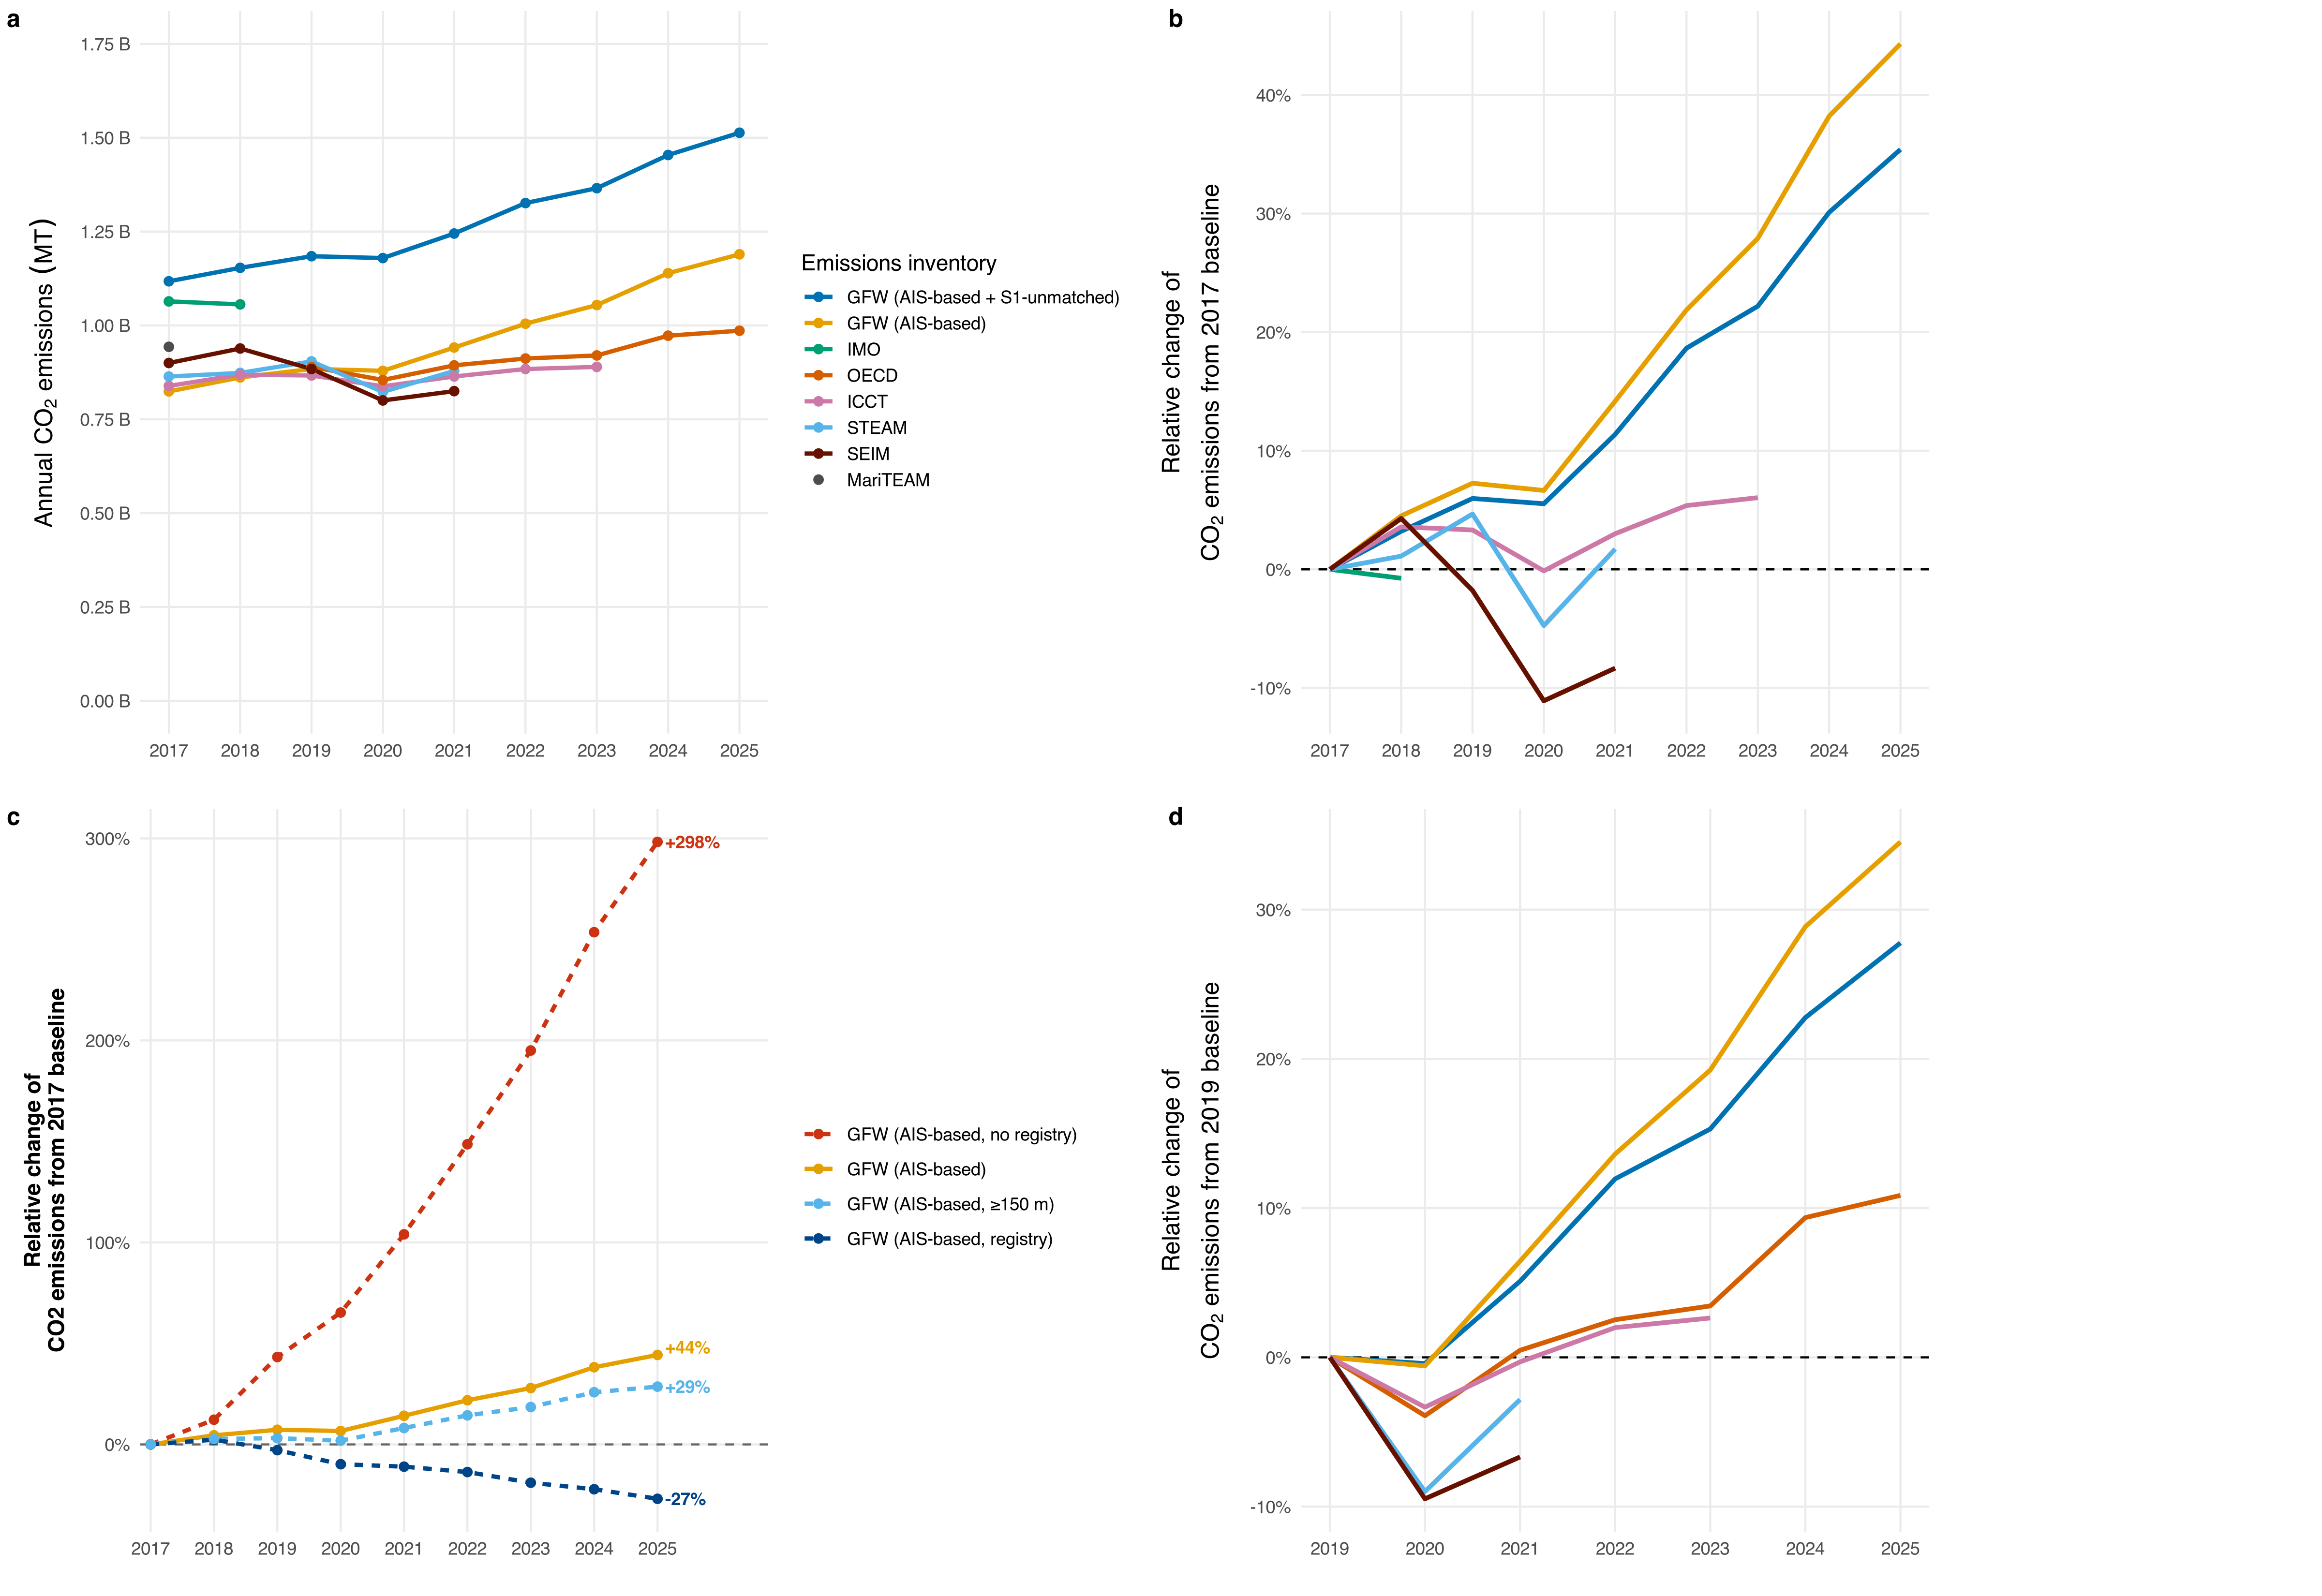
\includegraphics[width=\columnwidth,height=0.92\textheight,keepaspectratio]{figures/figS-inventory-comparison-all-sources-1.png}
    \caption{Our AIS and fused estimates against the published bottom-up inventories. Panel a shows levels; panels b and C show change relative to 2017 and 2019, respectively.}
    \label{fig:figS-inventory-comparison-all-sources}
\end{figure}

\begin{figure}[H]
    \centering
    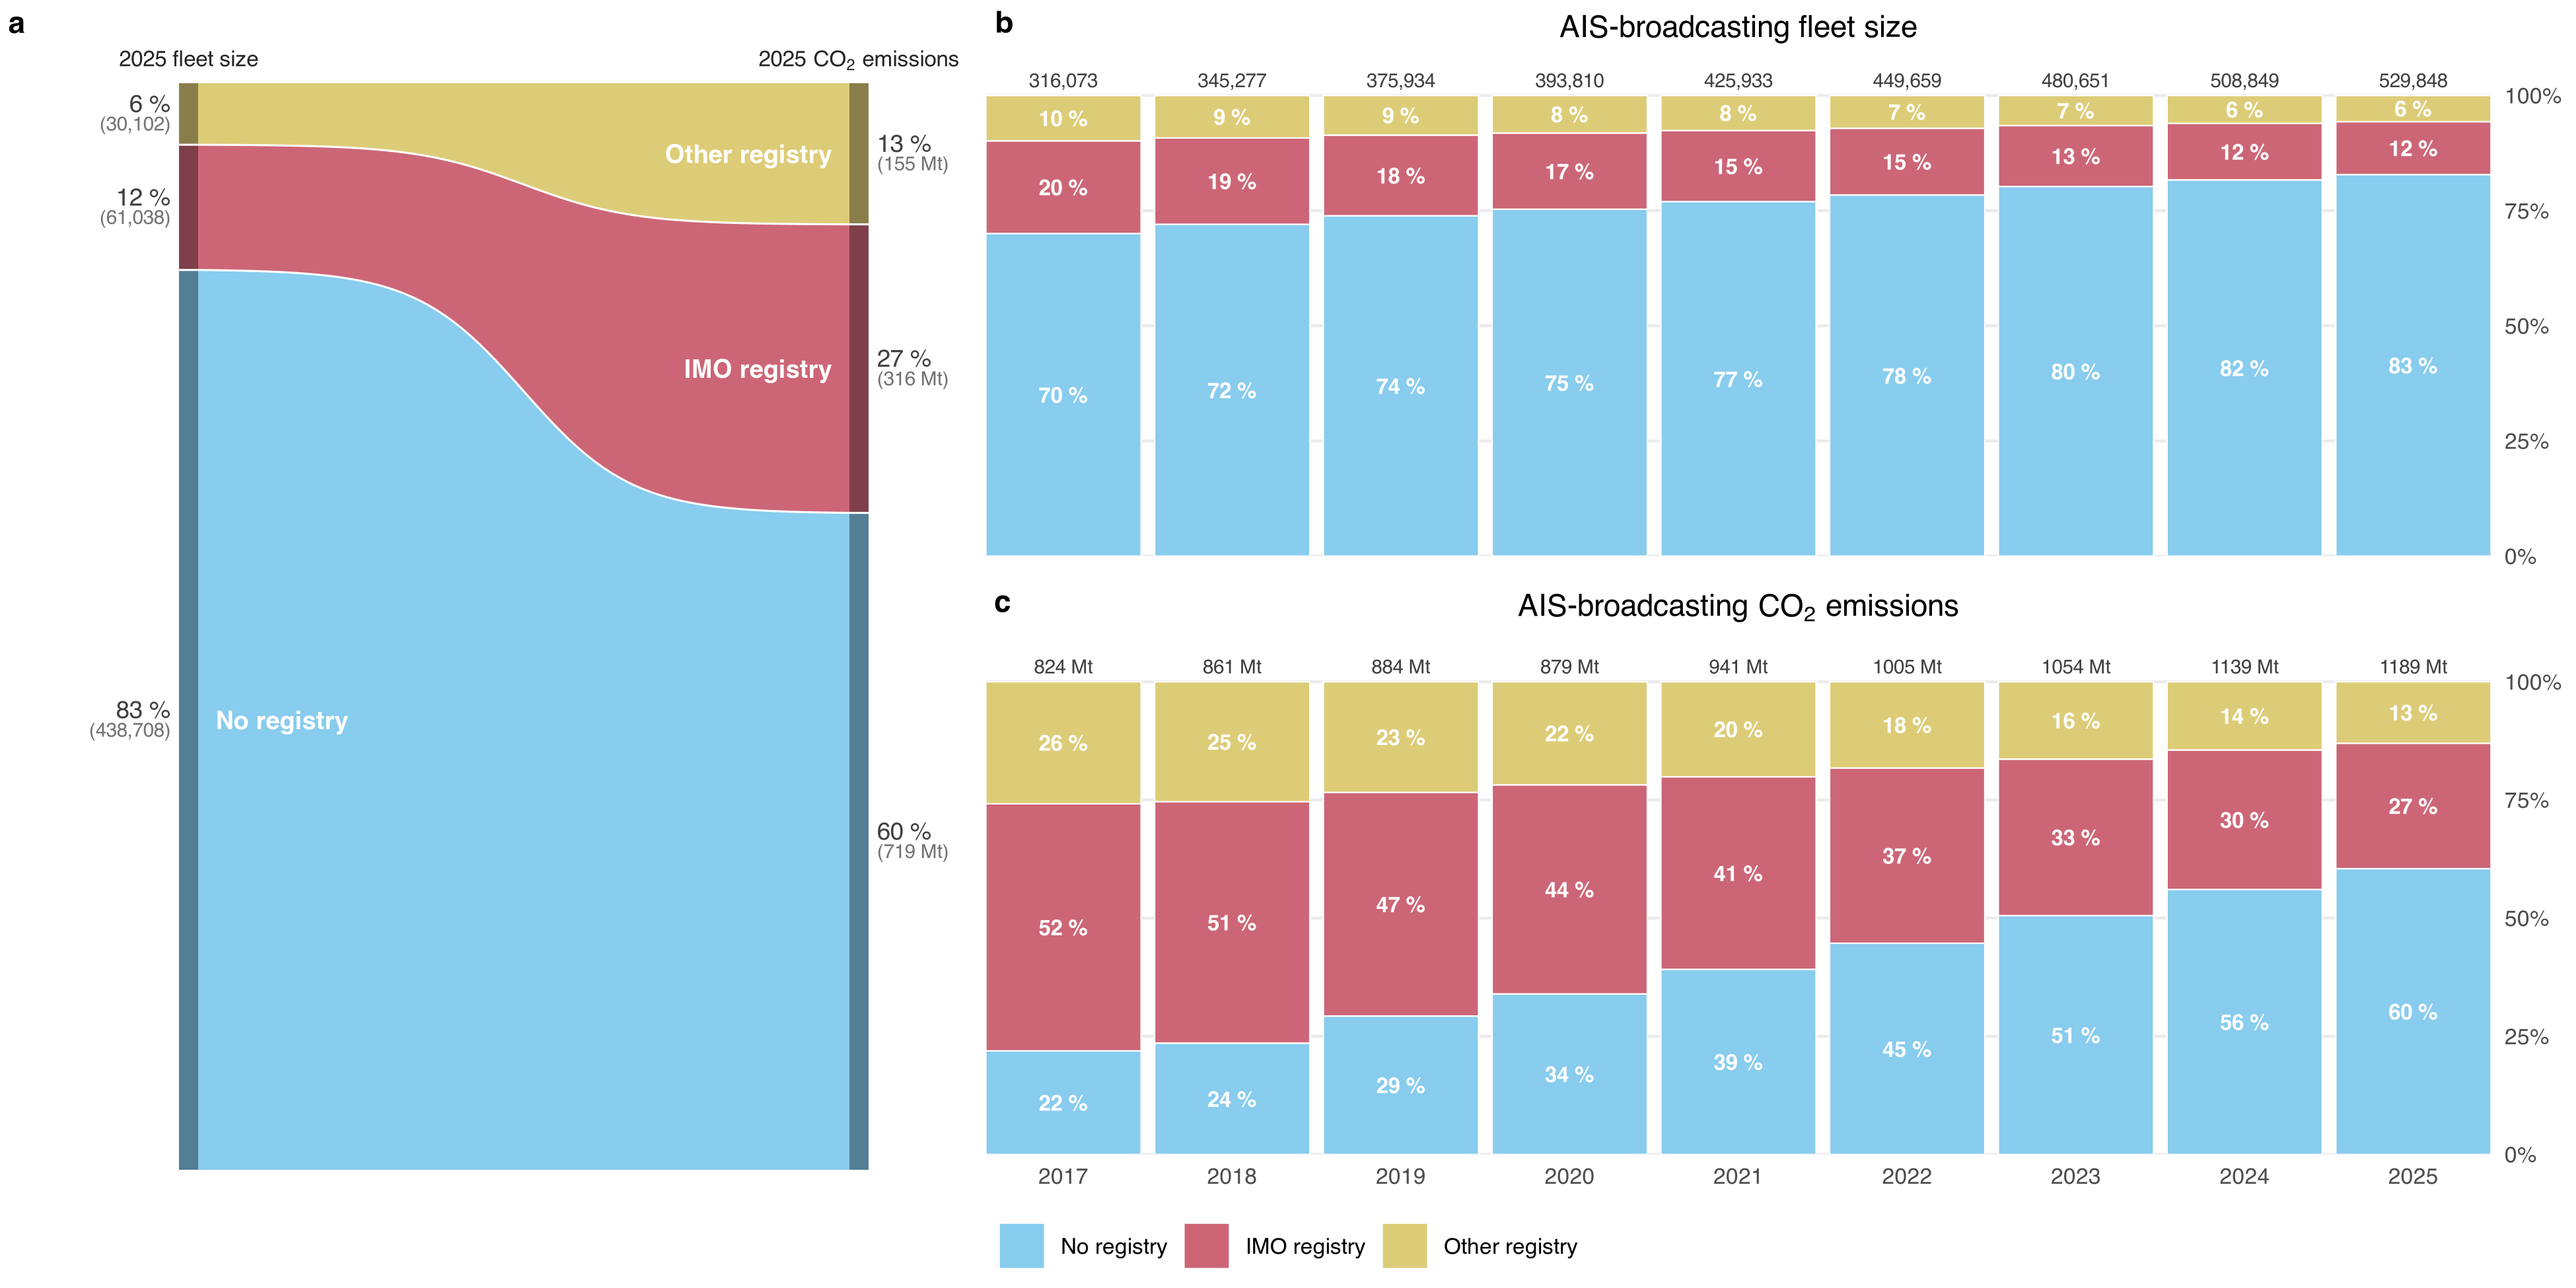
\includegraphics[width=\columnwidth]{figures/figS-registry-sankey-with-series-2025-1.png}
    \caption{Registry status in 2025: share of the fleet against share of CO$_{2}$ for registry-matched and unmatched vessels, with the supporting series.}
    \label{fig:figS-registry-sankey-with-series-2025}
\end{figure}

% Nine columns overflow the text block at the default column padding
\begingroup
\setlength{\tabcolsep}{2.5pt}
\begin{table}[!h]
\centering
\caption{\label{tab:inventory_comparison_all_sources}Annual marine vessel CO$_{2}$ emissions (billions of metric tonnes) for our AIS-based and fused (AIS-based + S1-unmatched) estimates and for the published bottom-up, activity-based inventories. A dash marks a year for which an inventory publishes no estimate.}
\centering
\fontsize{7}{9}\selectfont
\setlength{\tabcolsep}{3pt}
\begin{tabular}[t]{r|l|l|l|l|l|l|l|l}
\hline
Year & \shortstack{GFW\\(AIS-based +\\S1-unmatched)} & \shortstack{GFW\\(AIS-based)} & IMO & OECD & SAVE & STEAM & SEIM & MariTEAM\\
\hline
2017 & 1.065 & 0.824 & 1.064 & - & 0.839 & 0.864 & 0.900 & 0.943\\
\hline
2018 & 1.098 & 0.861 & 1.056 & - & 0.869 & 0.874 & 0.939 & -\\
\hline
2019 & 1.128 & 0.884 & - & 0.889 & 0.867 & 0.904 & 0.884 & -\\
\hline
2020 & 1.122 & 0.879 & - & 0.855 & 0.838 & 0.823 & 0.800 & -\\
\hline
2021 & 1.187 & 0.941 & - & 0.894 & 0.864 & 0.879 & 0.825 & -\\
\hline
2022 & 1.259 & 1.005 & - & 0.912 & 0.884 & - & - & -\\
\hline
2023 & 1.299 & 1.054 & - & 0.920 & 0.890 & - & - & -\\
\hline
2024 & 1.384 & 1.139 & - & 0.973 & - & - & - & -\\
\hline
2025 & 1.443 & 1.189 & - & 0.986 & - & - & - & -\\
\hline
\end{tabular}
\end{table}

\endgroup
\FloatBarrier

Two subsequent changes drive the divergence in our emissions estimates that follows in the most recent years. First, our AIS-broadcasting fleet grows faster than the OECD and SAVE fleets, the only inventories with vessel-count series overlapping the recent period (Fig. \ref{fig:figS-inventory-vessel-counts-by-registry}). These contrasting trends likely reflect differences in how each fleet is constructed (Table \path{bottom-up_inventory_comparison_inputs.csv}). Inventories that are more constrained by commercial registries (even when they also consider to some extent non-registered vessels) change primarily at the pace of registry updates. Our fleet, by contrast, is more AIS observation-driven where both the number and the share of vessels that cannot be matched to a registry rose over time carrying all the increase in emissions (Fig. \ref{fig:figS-registry-sankey-with-series-2025} and Fig. \ref{fig:figS-registry-split-comparison}). Our trends are therefore conditioned more by the expansion of AIS carriage than are those of other inventories, all of which rely more heavily than ours on registry-based fleet definitions holding their emissions more constant (Fig. \ref{fig:figS-inventory-comparison-all-sources}, panel b and C). S1 detections make this directly observable. Among detected large non-fishing vessels—the segment where AIS carriage is mandated and registry coverage is strongest, and thus the closest analogue to a registry-based fleet—the share that cannot be matched to an AIS broadcast is essentially unchanged since 2017, whereas that share falls steeply among small non-fishing and fishing vessels as AIS carriage and reception expand (Fig. \ref{fig:figS-ais-carriage-saturation-by-size}).

\begin{figure}[H]
    \centering
    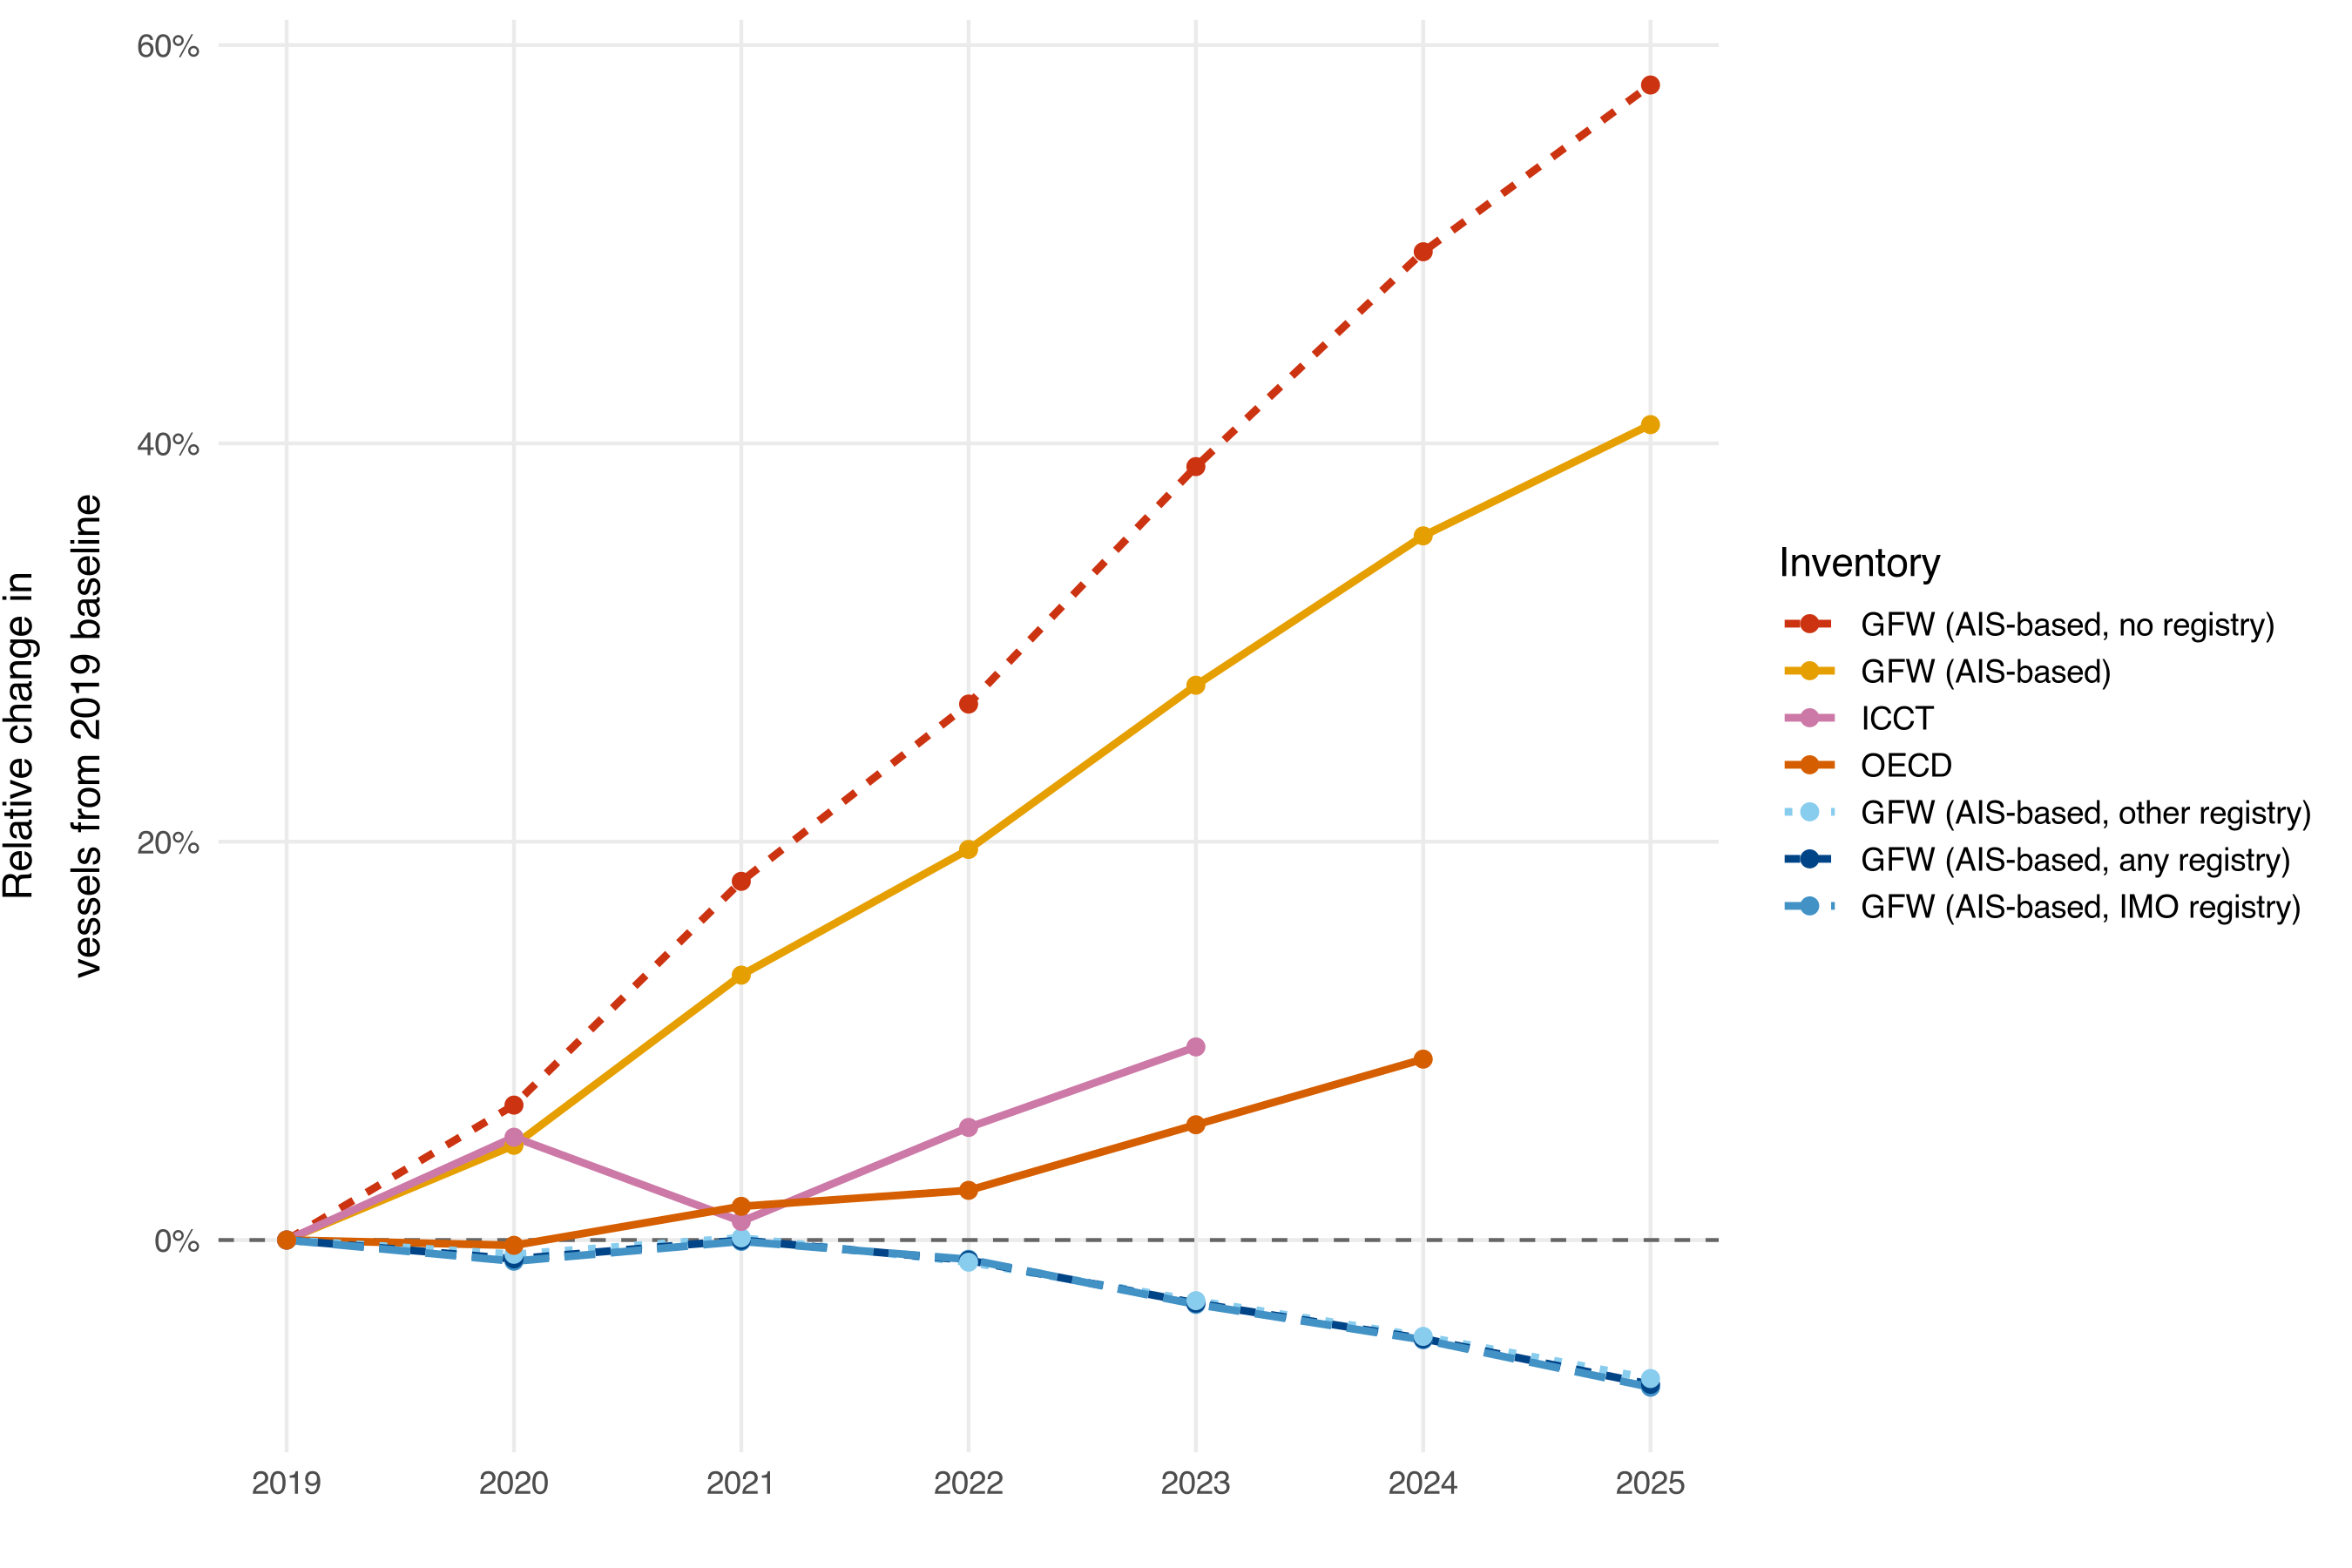
\includegraphics[width=\columnwidth]{figures/figS-inventory-vessel-counts-by-registry-1.png}
    \caption{Modelled fleet size over time for the inventories publishing a vessel count per year, split by registry status for ours.}
    \label{fig:figS-inventory-vessel-counts-by-registry}
\end{figure}

\begin{figure}[H]
    \centering
    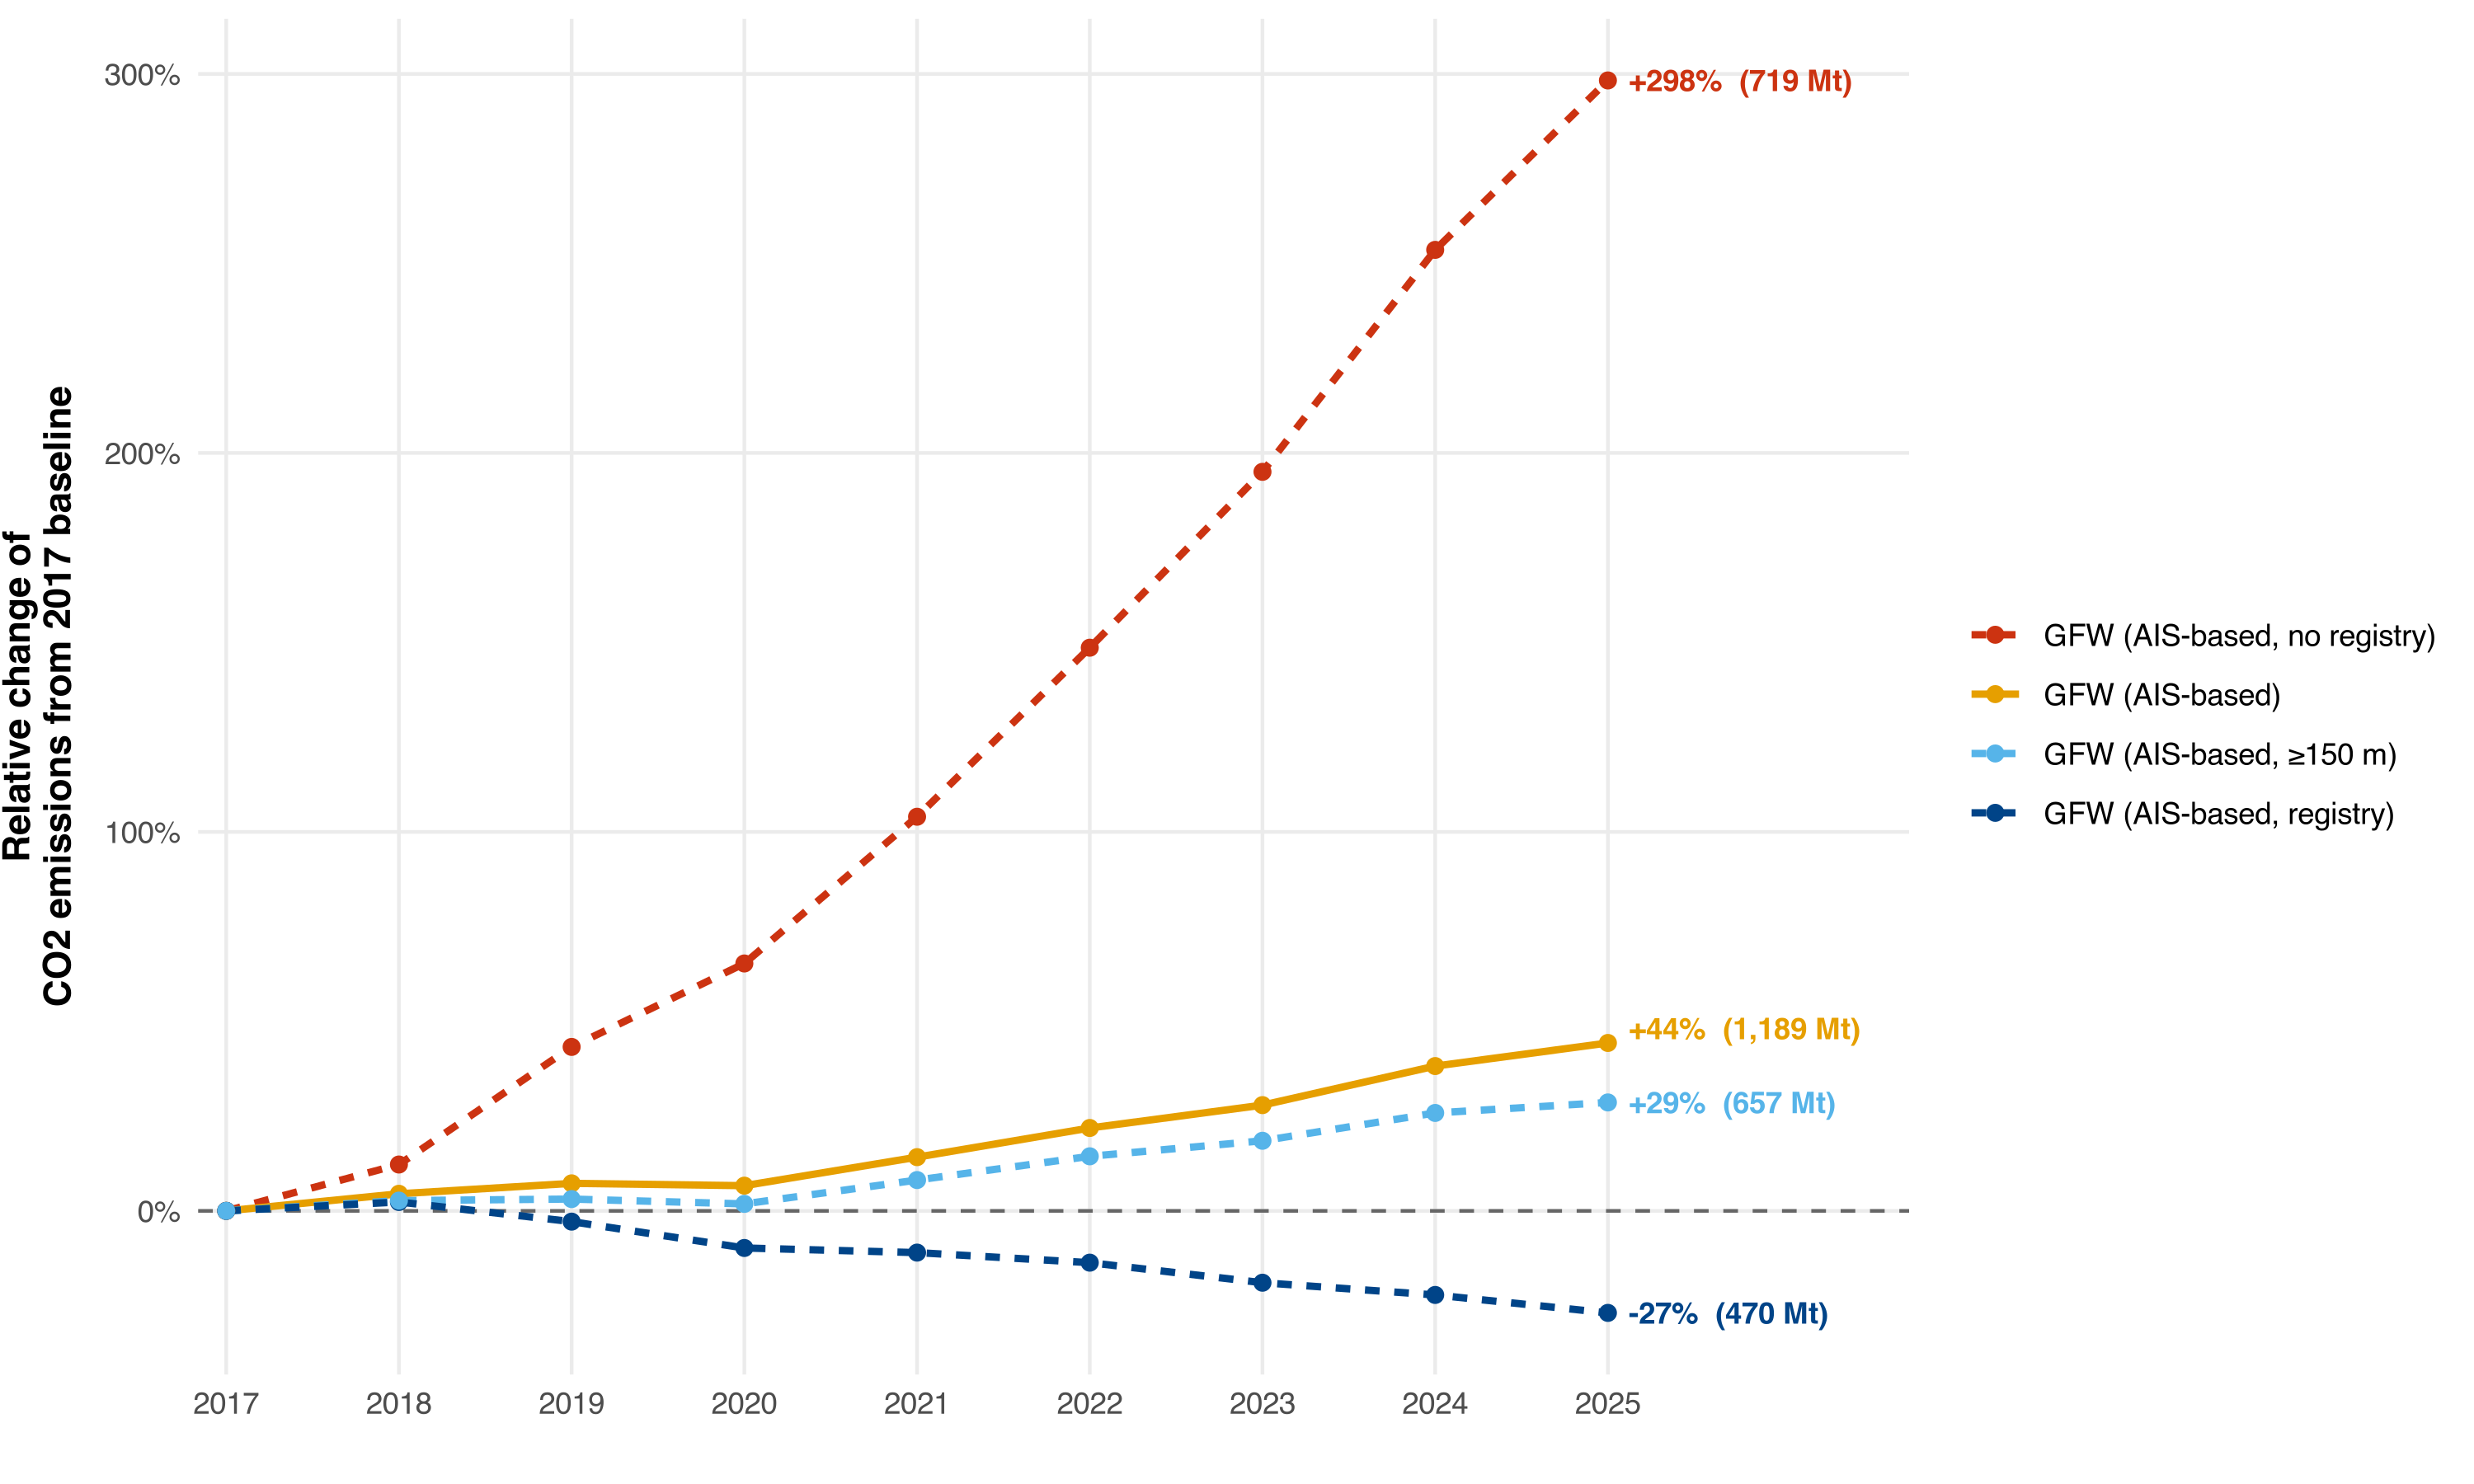
\includegraphics[width=\columnwidth]{figures/figS-registry-split-comparison-1.png}
    \caption{Emissions from registry-matched and unmatched vessels, relative to 2017, with the size-restricted fragment for comparison.}
    \label{fig:figS-registry-split-comparison}
\end{figure}

\begin{figure}[H]
    \centering
    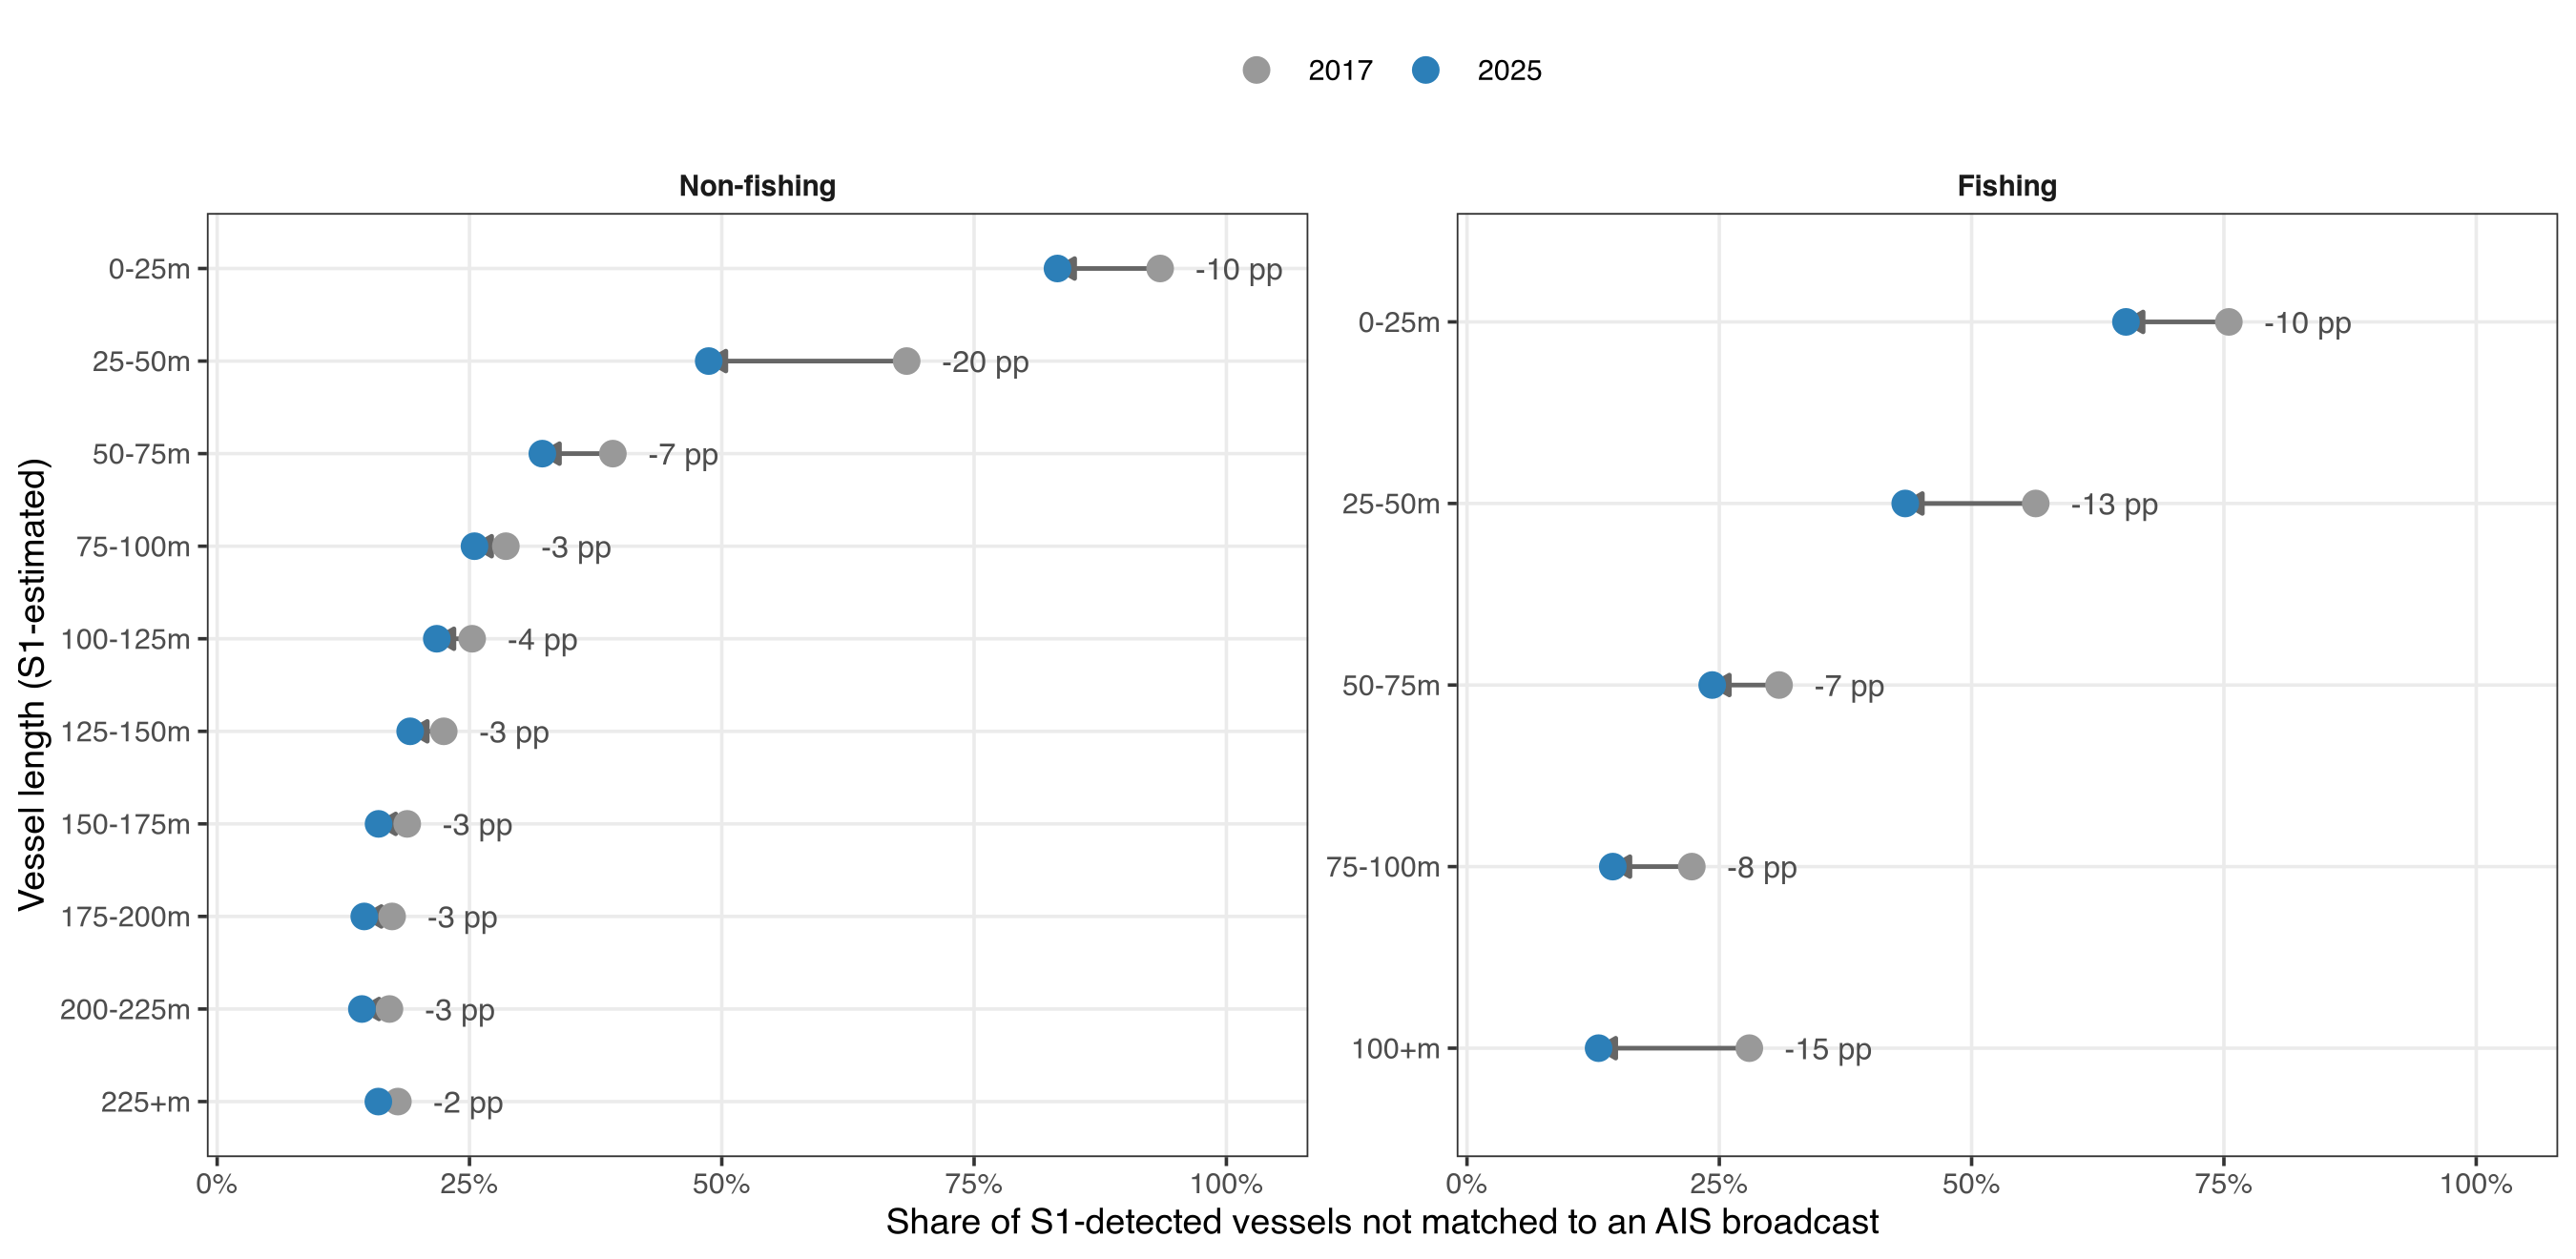
\includegraphics[width=\columnwidth]{figures/figS-ais-carriage-saturation-by-size-1.png}
    \caption{AIS carriage saturation by vessel size: the unmatched share is flat for the largest vessels and falls steeply for the smallest.}
    \label{fig:figS-ais-carriage-saturation-by-size}
\end{figure}

Second, our observed activity is also shaped by the phase-in of dynamic AIS (D-AIS), after which the emissions gap to the other inventories widens most rapidly (Fig. \ref{fig:figS-inventory-comparison-all-sources}). D-AIS primarily increases AIS-estimated emissions where it fills gaps that were previously unobserved, particularly in high-traffic zones where satellite reception degrades. Activity that was formerly interpolated across, or missed altogether, becomes measured, adding newly observable emissions to the inventory. Alongside this, D-AIS also acts on resolution, densifying segments that were already observed so that trajectories are more tightly constrained and speed profiles better resolved, without additional activity entering the inventory. Both mechanisms operate, but the second predominates: AIS positions received more than double between 2021 and 2025, while observed distance travelled and AIS emissions rise together by only $\sim$27\%, with emissions per message falling accordingly (Fig. \ref{fig:figS-messages-vs-hours-vs-emissions}). Densification also improves S1 detection-AIS matching, so where this occurs activity moves from the modelled dark component to the AIS one, and its emissions get computed directly from AIS rather than estimated by the dark model, a reallocation between the fused components rather than an addition.

\begin{figure}[H]
    \centering
    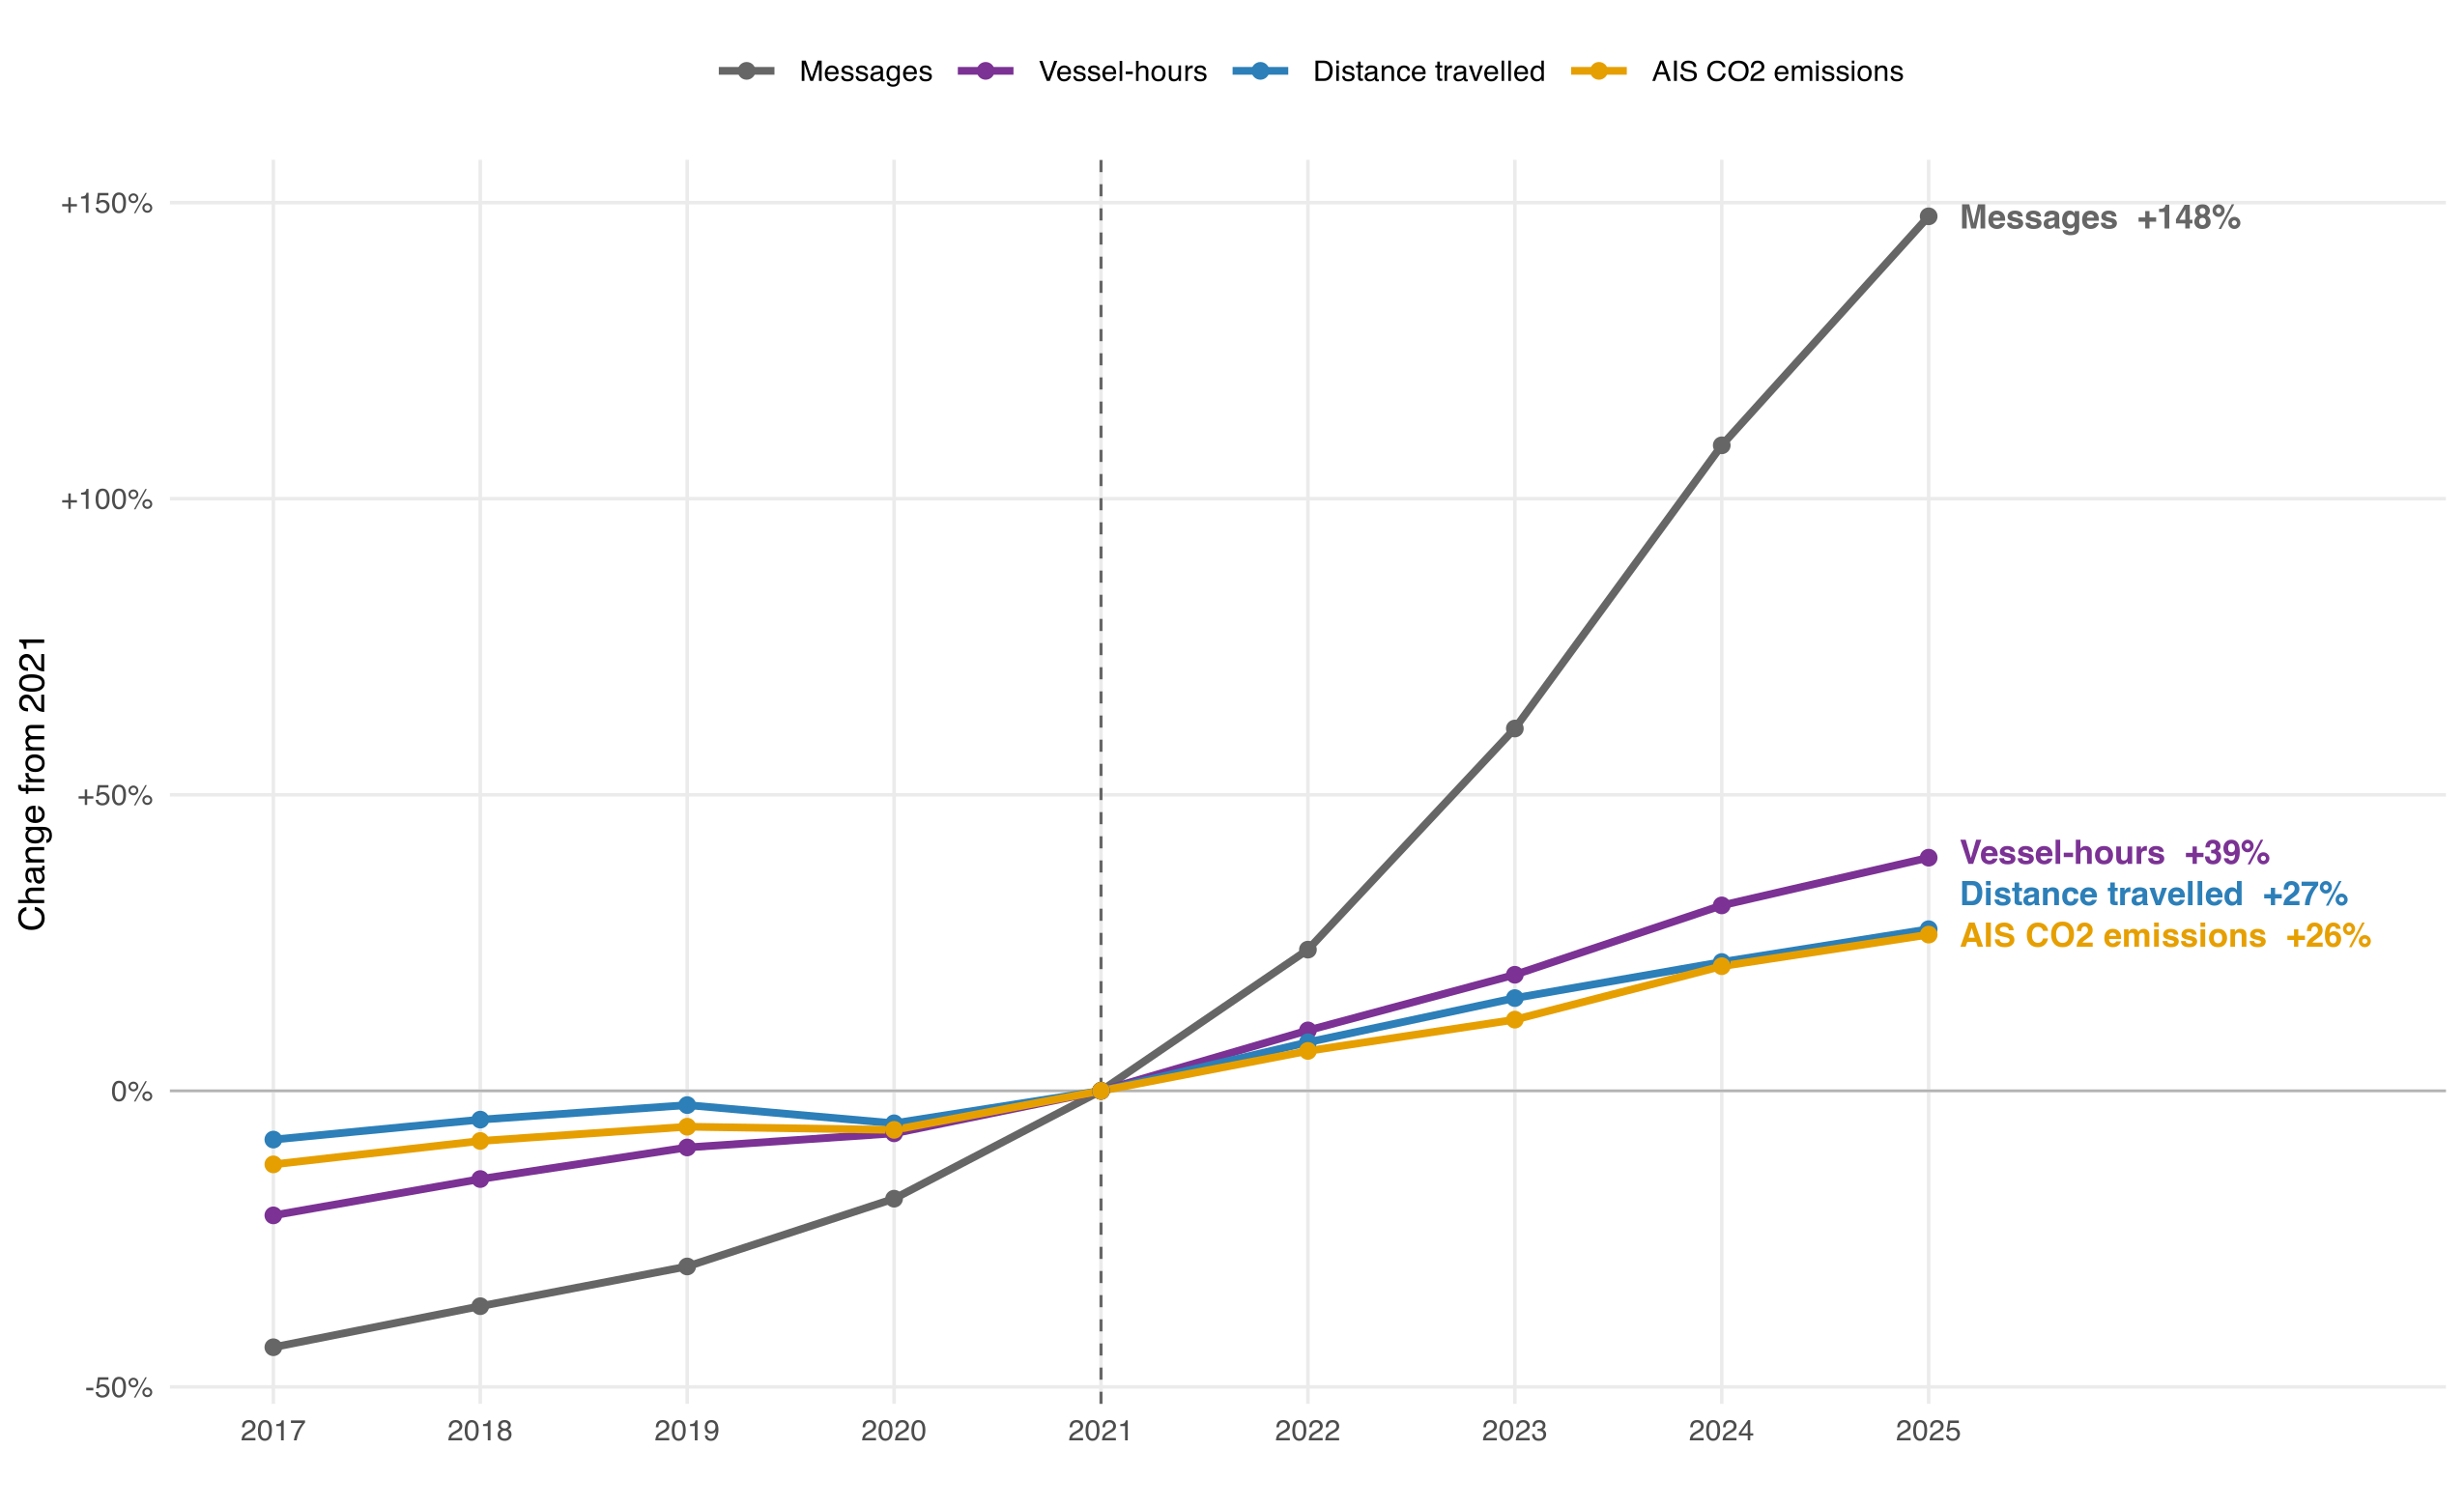
\includegraphics[width=\columnwidth]{figures/figS-messages-vs-hours-vs-emissions-1.png}
    \caption{AIS messages received against observed activity and emissions, indexed to 2021, separating densification from new activity.}
    \label{fig:figS-messages-vs-hours-vs-emissions}
\end{figure}

The above suggests that the increase in emissions occurs mostly via AIS carriage and, to a lesser extent, AIS coverage. The emissions divergence against the other inventories therefore does not indicate that our totals are inflated—a conclusion also supported by our global per-vessel emissions and emission intensities relative to other models (Table \ref{tab:inventory_intensity_all_models})—but rather that the other inventories, and our own early years, are missing part of the fleet and activity at sea. Global fleet emissions are likely understated wherever limited AIS carriage and/or high reliance on registry-defined fleets leaves low-information vessels out of the scope. This is supported by the S1 detection record where the share of detections that cannot be matched to an AIS broadcast has declined in all size classes since 2017, most steeply among fishing vessels and small non-fishing vessels, indicating an increase in AIS adoption (Fig. \ref{fig:figS-unmatched-fraction-fullperiod}). Indeed, the largest emissions growth we observe comes from passenger vessels, driven by the smallest group (Fig. \ref{fig:figS-passenger-size-panels}), and fishing vessels, a fleet segment comprising numerous small, largely coastal vessels that are poorly covered by registries and enter the model only as their AIS carriage expands (Fig. \ref{fig:figS-fleet-growth-by-year} and Fig. \ref{fig:figS-fleet-sankey-with-series-2025}). This is precisely the segment that registry-based methods are least equipped to capture.

\begin{figure}[H]
    \centering
    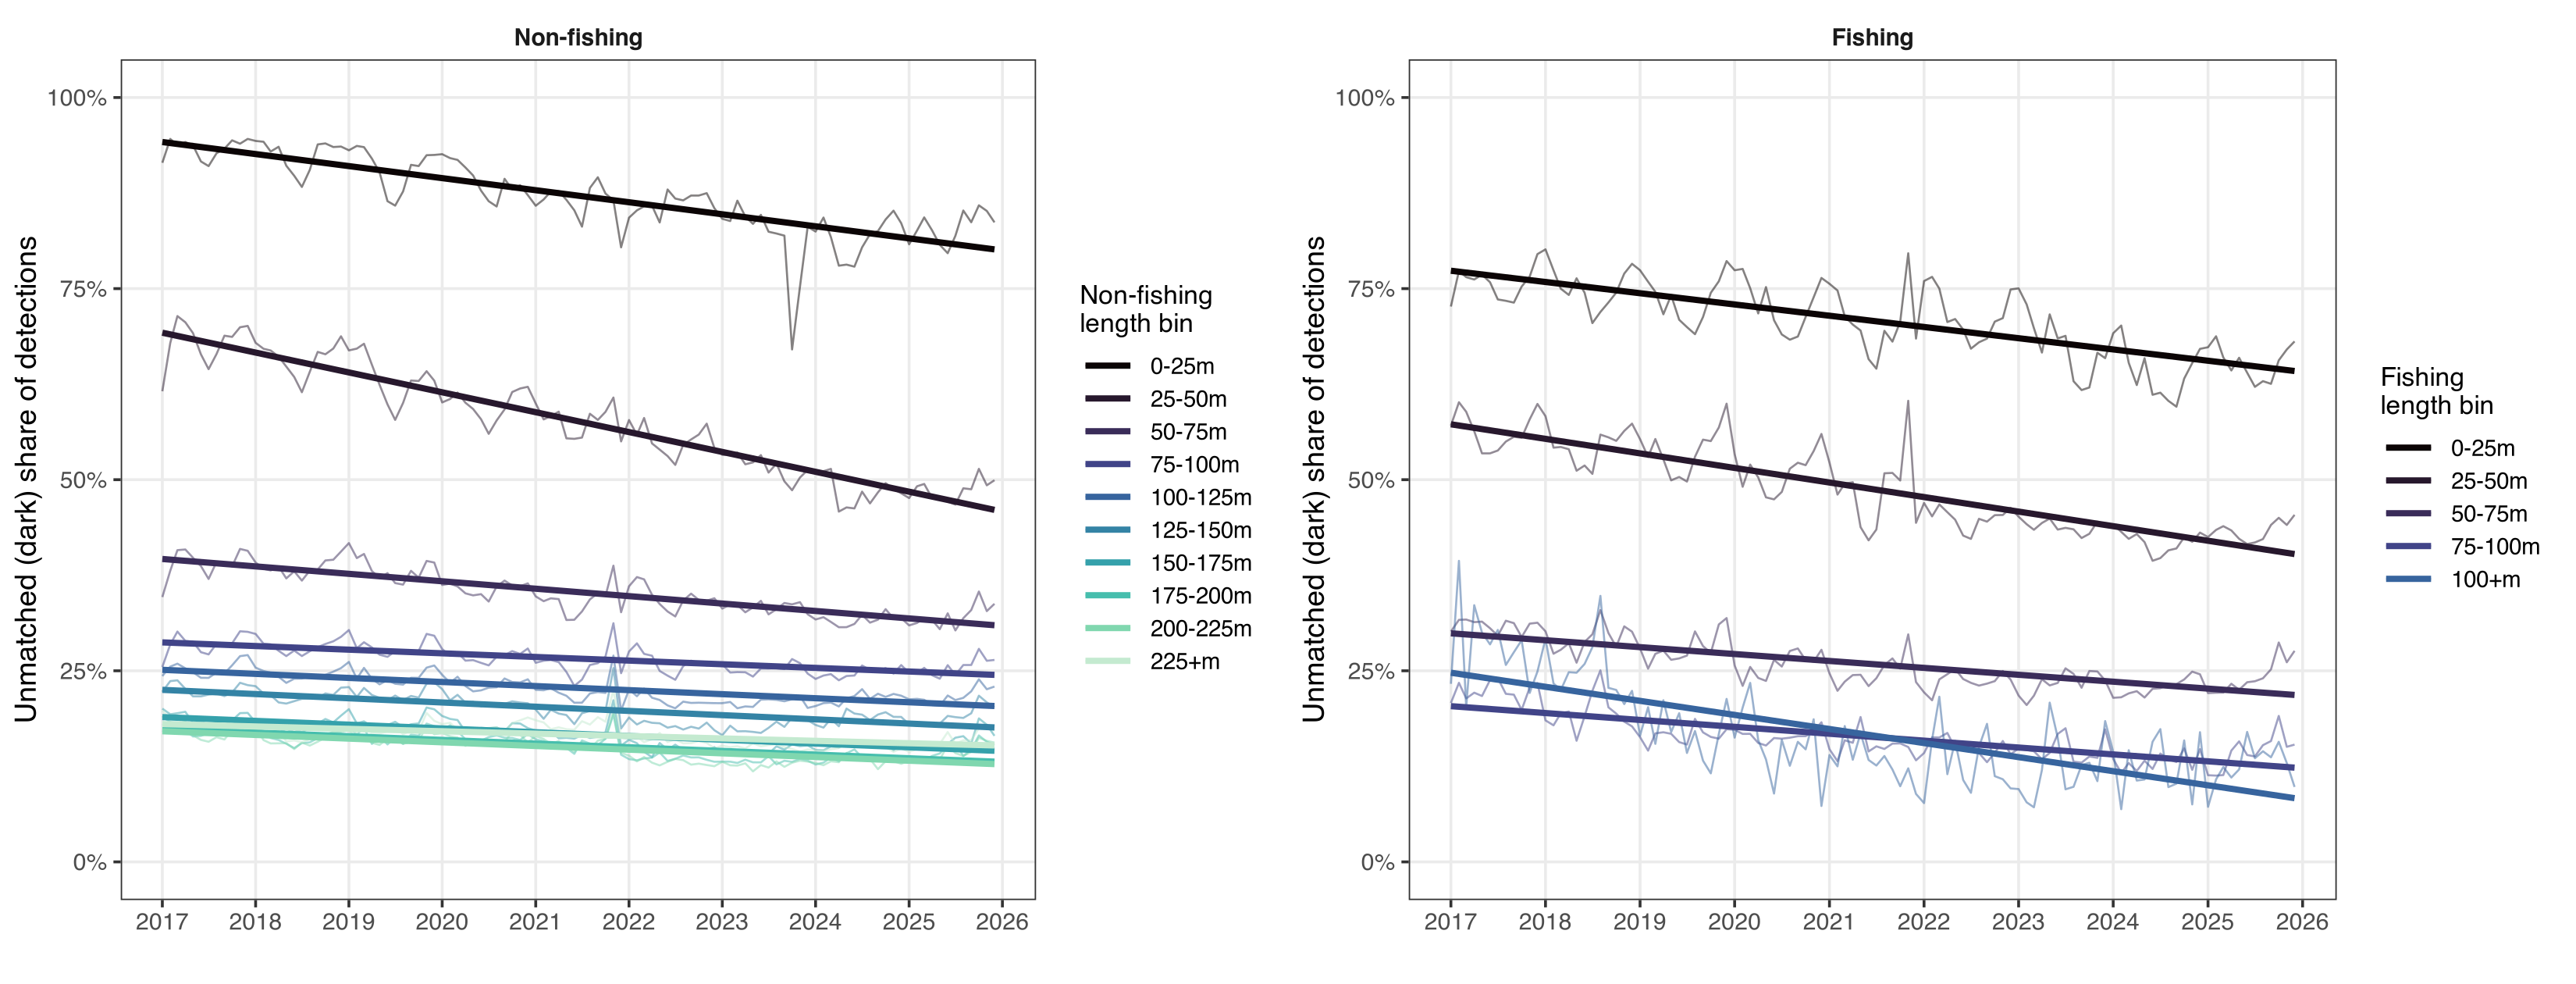
\includegraphics[width=\columnwidth]{figures/figS-unmatched-fraction-fullperiod-1.png}
    \caption{Share of S1 detections with no matching AIS broadcast, by length bin, over the full period.}
    \label{fig:figS-unmatched-fraction-fullperiod}
\end{figure}

\begin{figure}[!p]
    \centering
    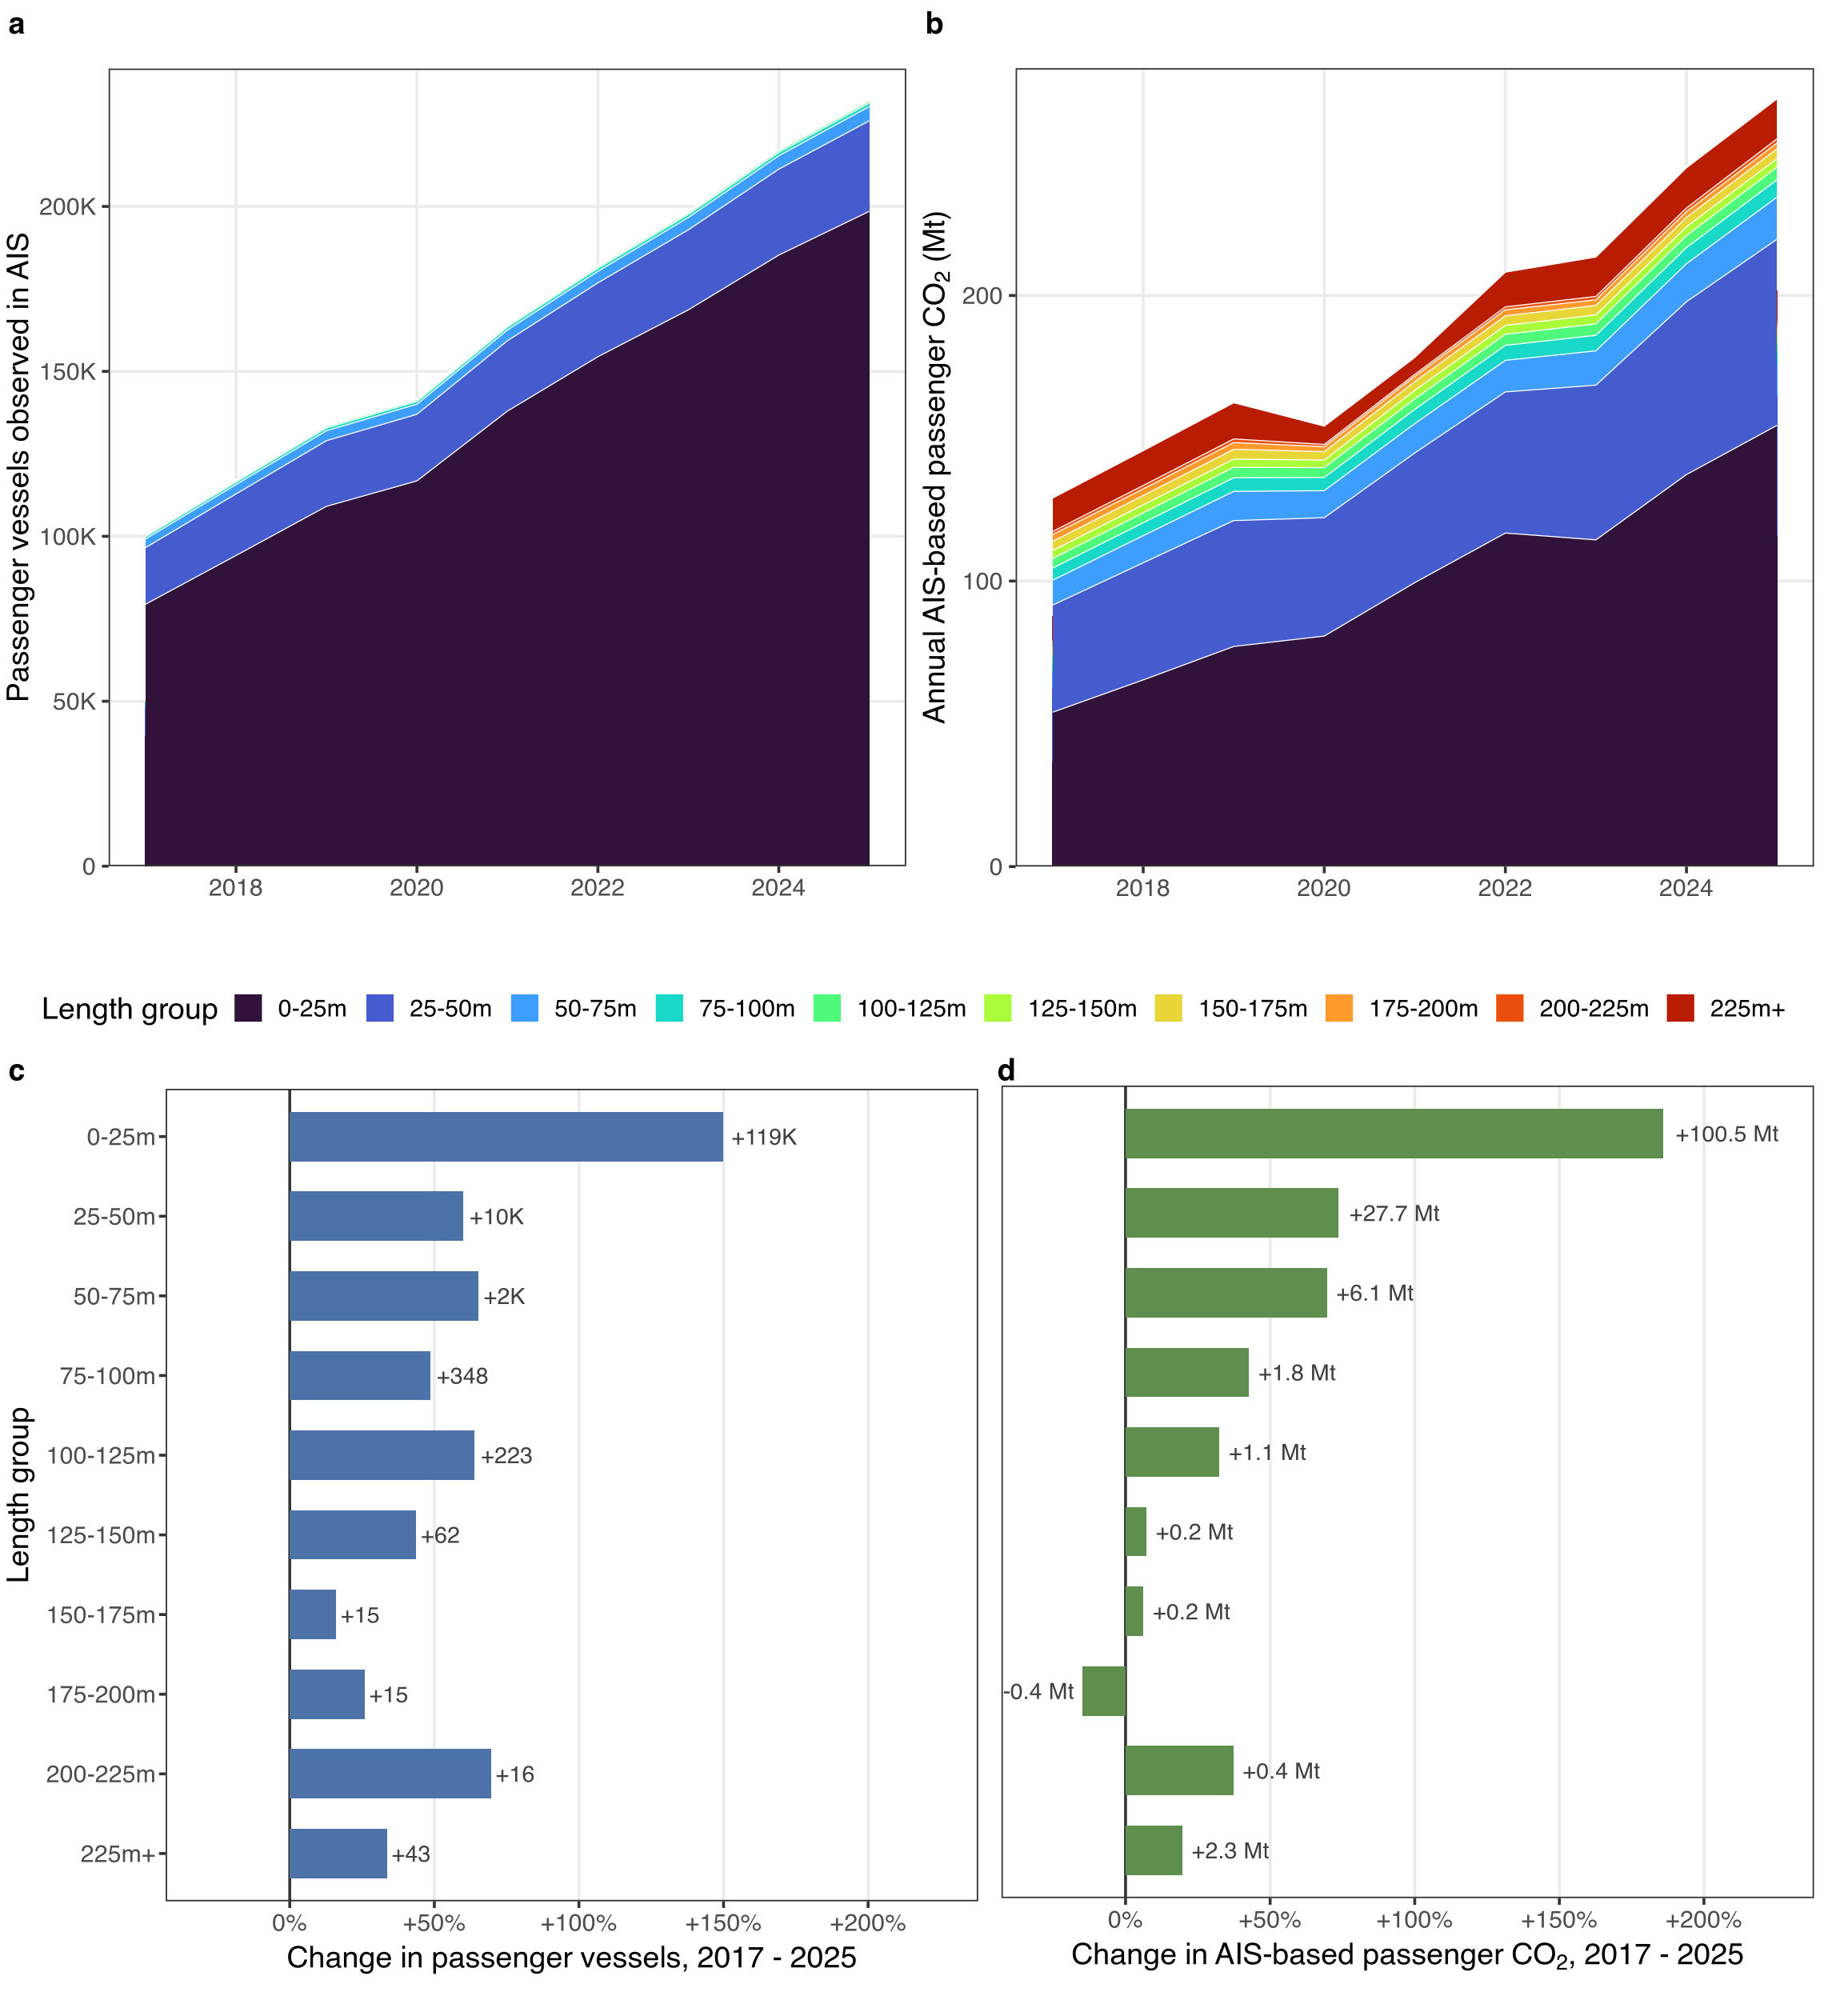
\includegraphics[width=\columnwidth,height=0.92\textheight,keepaspectratio]{figures/figS-passenger-size-panels-1.png}
    \caption{Passenger vessels by length bin, 2017 against 2025, showing growth concentrated in the smallest sizes.}
    \label{fig:figS-passenger-size-panels}
\end{figure}

\begin{figure}[H]
    \centering
    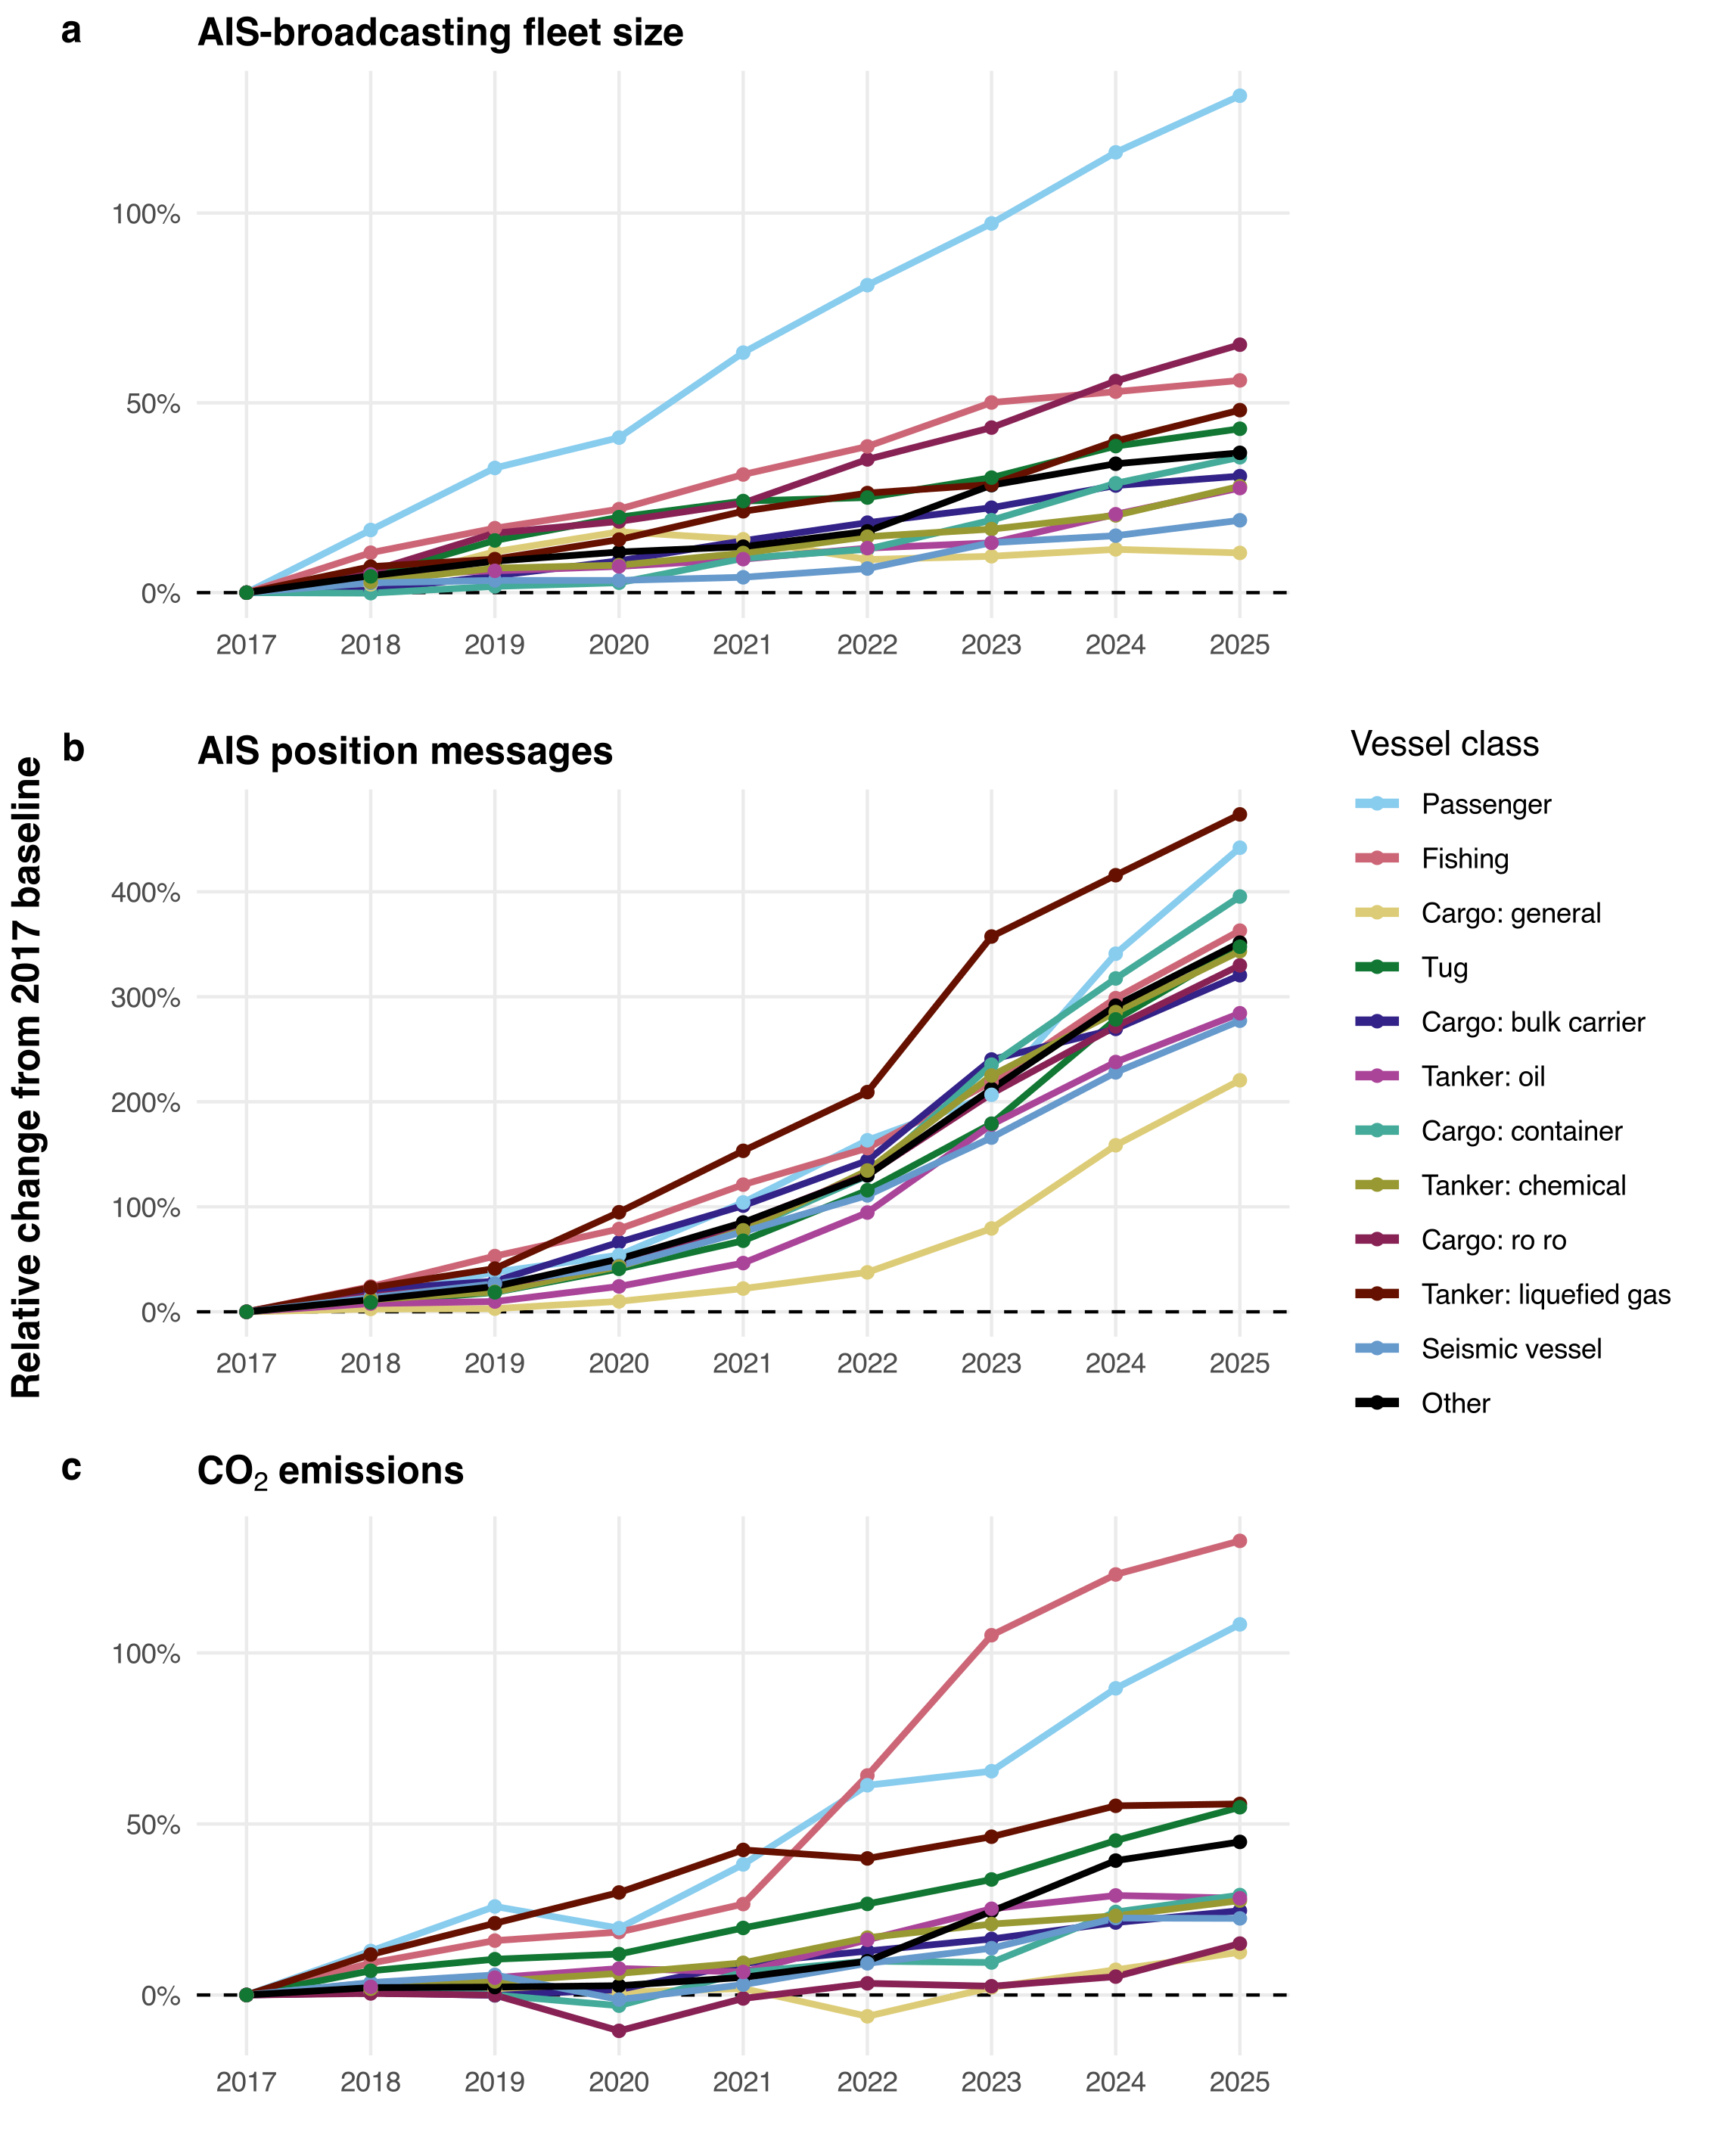
\includegraphics[width=\columnwidth]{figures/figS-fleet-growth-by-year-1.png}
    \caption{Growth by vessel class since 2017 in emissions, vessel count and activity.}
    \label{fig:figS-fleet-growth-by-year}
\end{figure}

\begin{figure}[H]
    \centering
    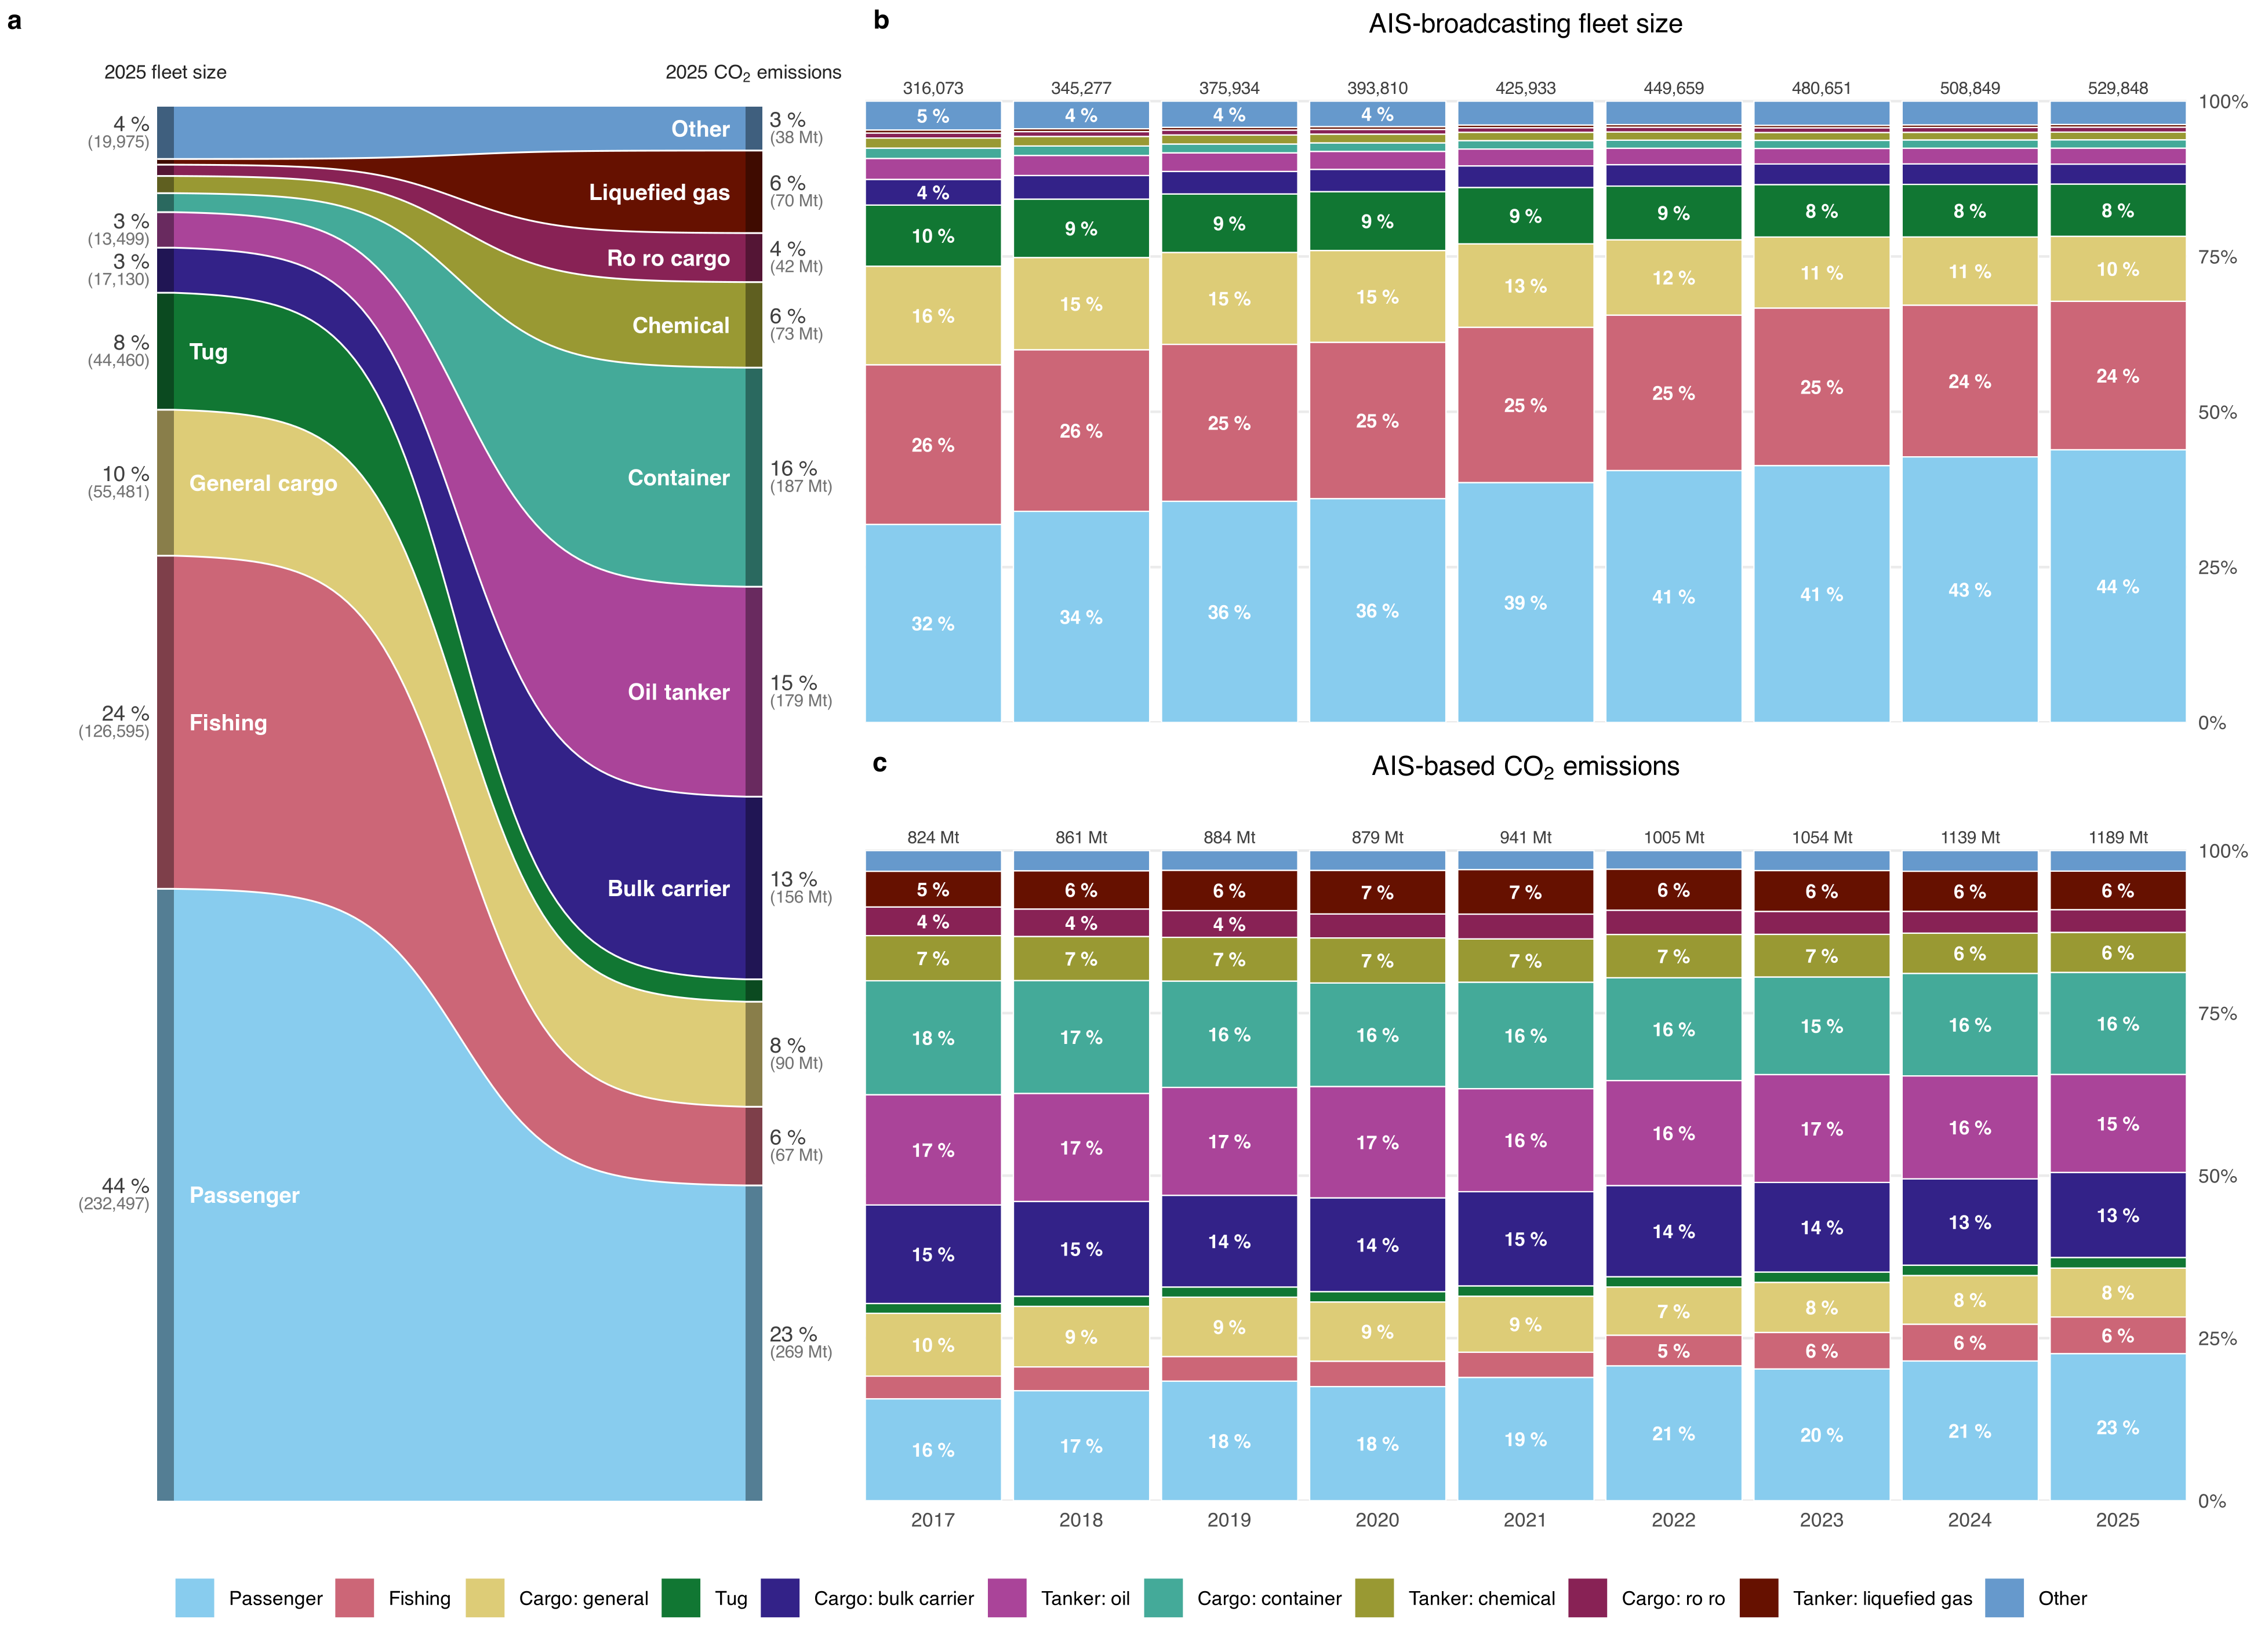
\includegraphics[width=\columnwidth]{figures/figS-fleet-sankey-with-series-2025-1.png}
    \caption{Fleet composition in 2025: each vessel class's share of the fleet against its share of CO$_{2}$, with the supporting series.}
    \label{fig:figS-fleet-sankey-with-series-2025}
\end{figure}

\begin{table}[!h]
\centering
\caption{\label{tab:inventory_intensity_all_models}CO$_2$ intensity per vessel for each inventory in the comparison, ordered by intensity. Intensities are computed on the fleet count each model publishes: single-total models use their reported figure, per-year models the mean over years where both a count and emissions exist, and the GFW rows our own activity summary on the same basis. Per-distance intensity is shown only for the models reporting distance travelled: ICCT restricted to its distance-reporting classes, and our AIS series whole and registry-matched.}
\centering
\fontsize{8}{10}\selectfont
\begin{tabular}[t]{lrr}
\toprule
Inventory & CO$_2$ per vessel (kt) & CO$_2$ per distance (kg nm$^{-1}$)\\
\midrule
MariTEAM & 20.55 & ---\\
SEIM & 7.90 & ---\\
OECD & 7.83 & ---\\
ICCT (distance-reporting classes) & 6.78 & 289.5\\
GFW (AIS, any registry) & 6.08 & 317.8\\
\addlinespace
IMO & 4.92 & ---\\
ICCT & 3.39 & ---\\
GFW (AIS) & 2.34 & 322.4\\
STEAM & 2.33 & ---\\
\bottomrule
\end{tabular}
\end{table}

\FloatBarrier

Still, full coverage of vessel activity remains limited by what the modeling is anchored to, whether AIS transmissions or registry data. Our total estimates (summed across AIS-based and S1-unmatched emissions) extend the inventory through satellite imagery-based vessel detections, capturing vessels that appear in neither registries nor AIS records. As a result, emissions diverge even further from every other inventory across the entire time range (Fig. \ref{fig:figS-inventory-comparison-all-sources}). The Fourth IMO GHG Study, OECD, and SAVE also attempt to account for vessels with no AIS activity by assigning small registered vessels without AIS signals the activity profiles of explicitly modeled vessels. Yet only the IMO study approaches our total emissions. This again highlights the limits of anchoring an inventory to a registry, where its coverage can reach no further than the registry itself, blind both to the low-information segment of the fleet our AIS series captures and to the dark fleet beyond it.

\subsubsection{Comparing our estimates with top-down inventories}

We also compared our total estimates against two top-down inventories, the Emissions Database for Global Atmospheric Research (EDGAR) and the Community Emissions Data System (CEDS). EDGAR builds its shipping estimates from reported fuel sales, representing international shipping from international marine bunkers and domestic activity from domestic navigation fuel statistics, with recent years extrapolated from Energy Institute fuel oil trends \cite{guizzardiGlobalUptoDate2025}. EDGAR can therefore only count fuel that was sold and reported. CEDS also starts from reported fuel sales but treats them as incomplete, on the view that marine fuel is systematically underreported, and raises its global shipping total using bottom-up estimates, mainly from the IMO GHG Studies \cite{hoeslyHistorical17502014Anthropogenic2018, ceds_data_and_assumptions}. Its limits are therefore not only what gets sold, but also the coverage of the bottom-up studies its global total rests on, whose limitations were described in the previous section.

Our total estimates (summed across AIS-based and S1-unmatched emissions) exceed both inventories, each of which is bounded by the fleet and activity they can resolve (Fig. \ref{fig:figS-multisector-shipping-comparison}, tabulated in Table \ref{tab:multisector_shipping_comparison}). The differences are in magnitude and in trend, reflecting differences in fleet scope and composition, respectively.

\begin{figure}[H]
    \centering
    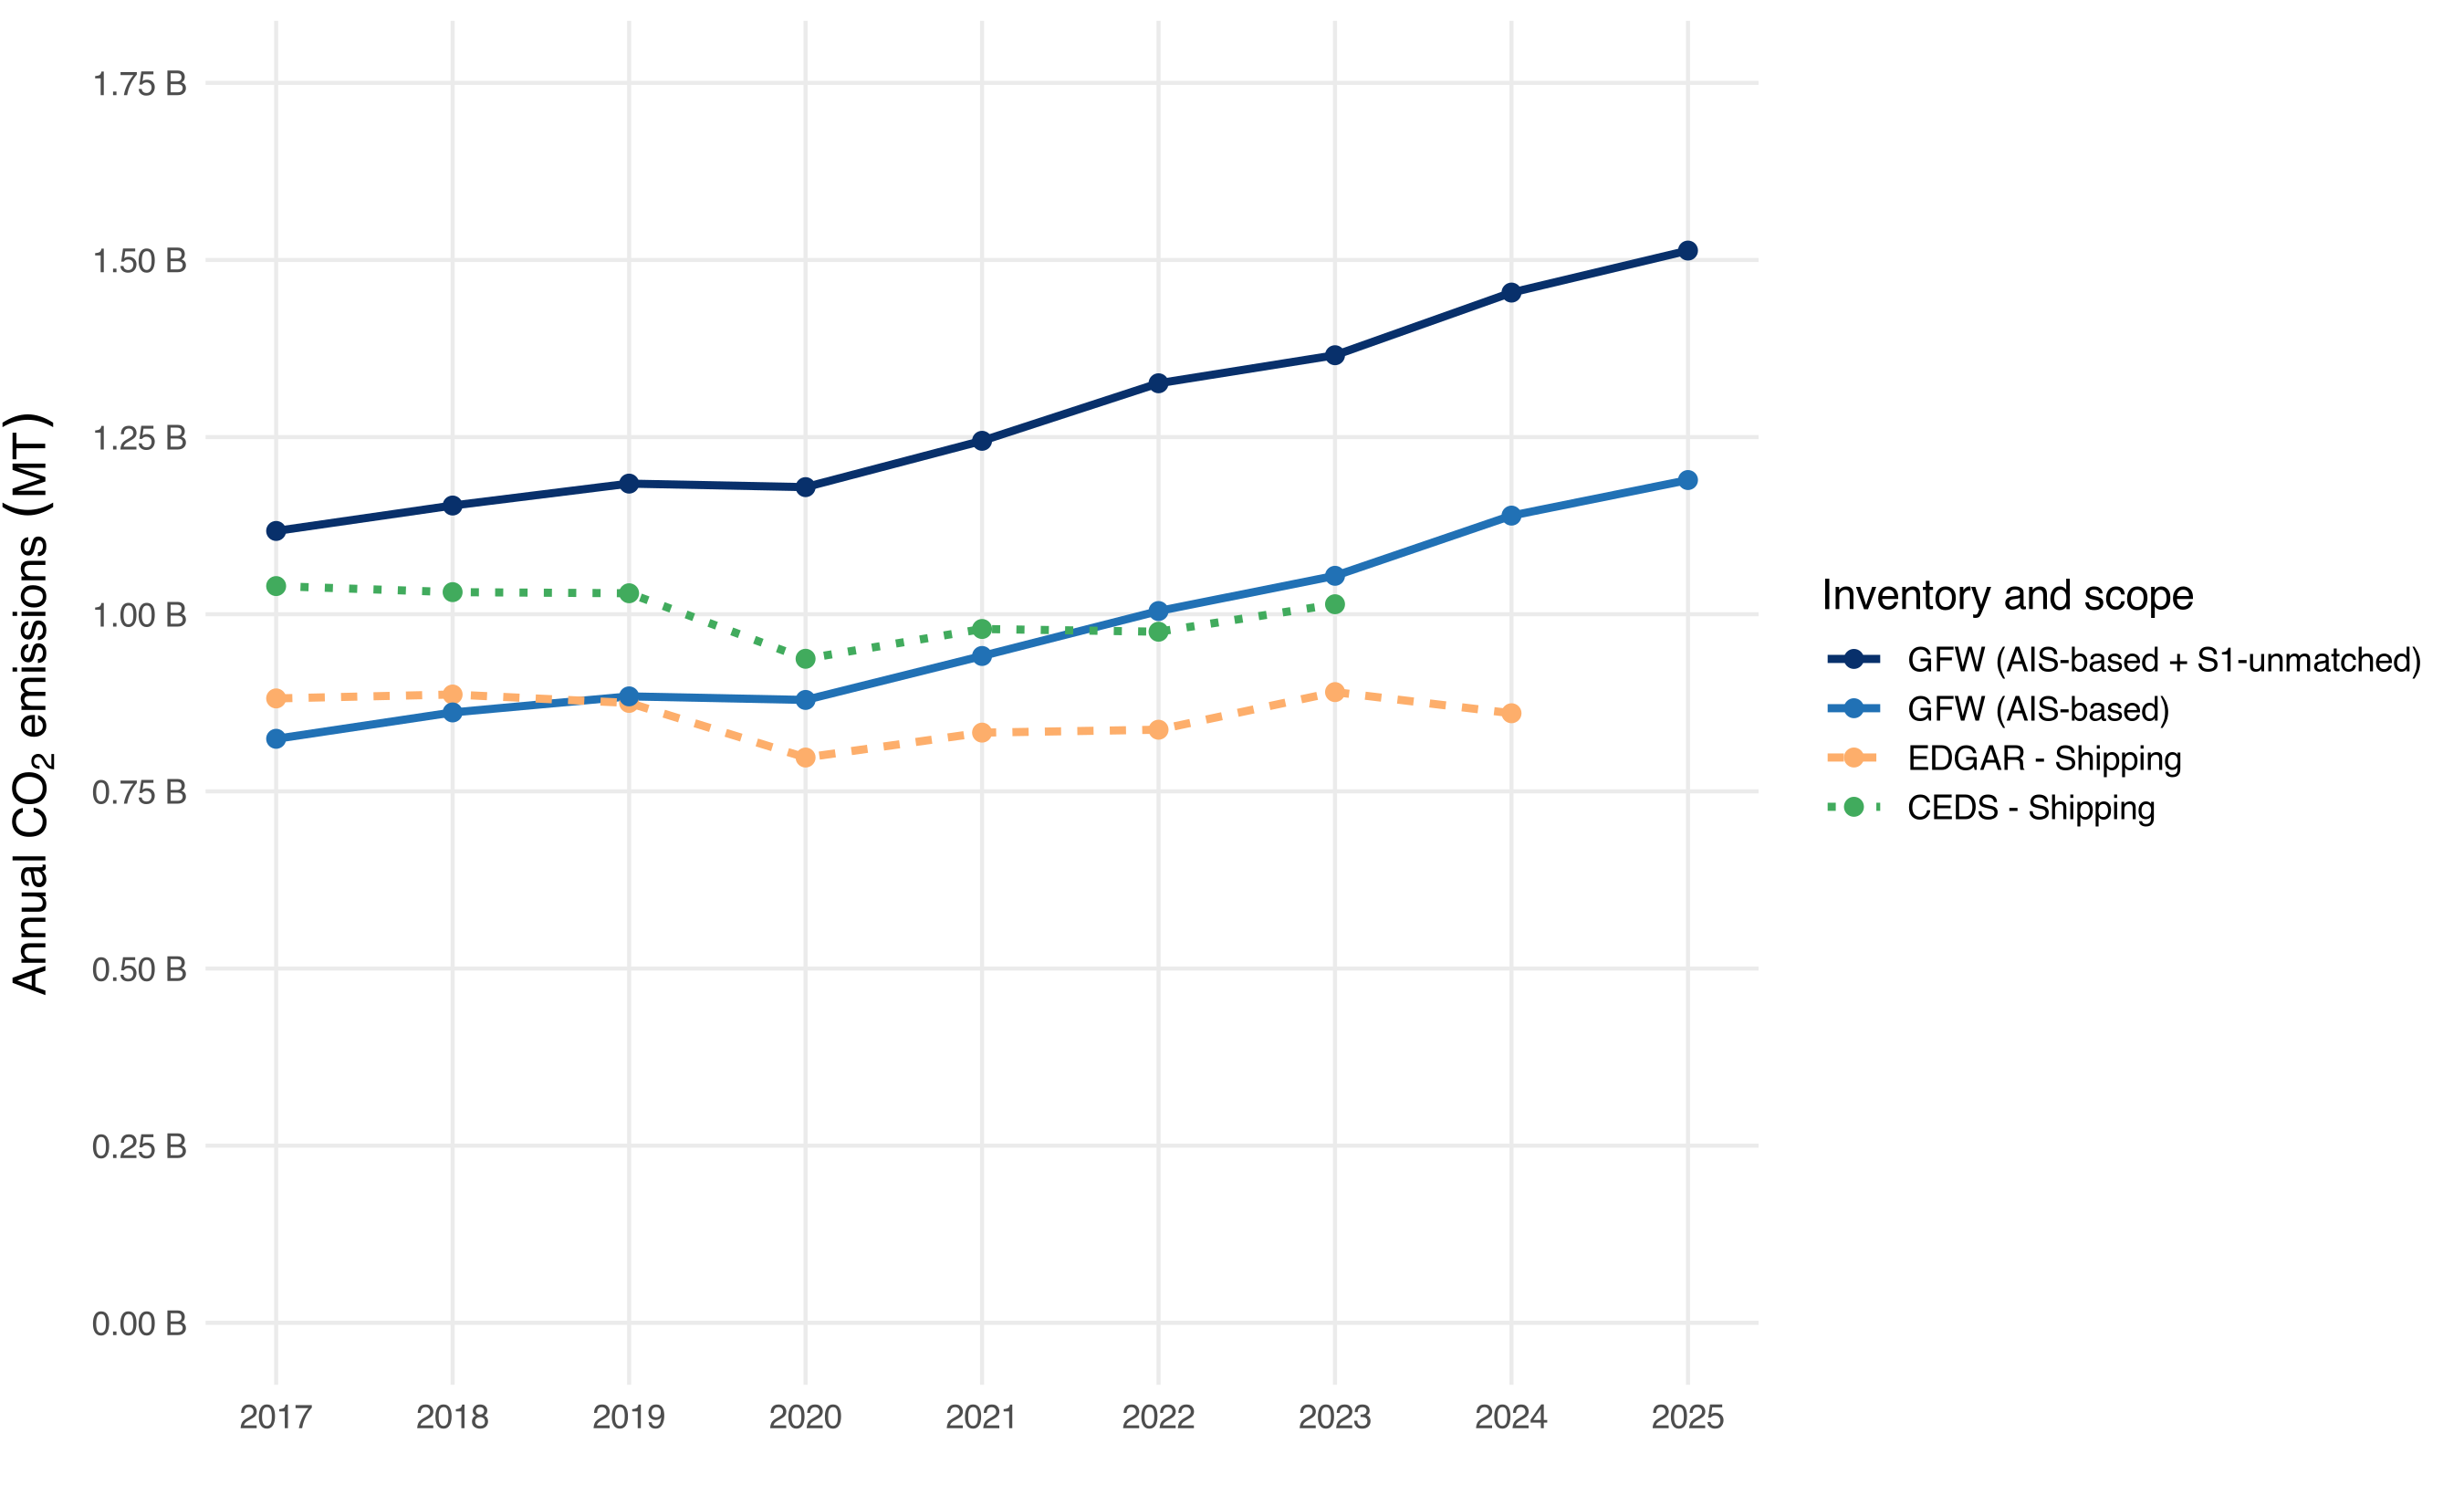
\includegraphics[width=\columnwidth]{figures/figS-multisector-shipping-comparison-1.png}
    \caption{Our shipping totals against the shipping sector of the top-down EDGAR and CEDS inventories.}
    \label{fig:figS-multisector-shipping-comparison}
\end{figure}

\begin{table}[!h]
\centering
\caption{\label{tab:multisector_shipping_comparison}Annual marine vessel CO$_{2}$ emissions (billions of metric tonnes) for our AIS-based and fused (AIS + S1) estimates against the shipping sector of the top-down EDGAR and CEDS inventories, whose shipping scope combines international and domestic navigation. A dash marks a year for which an inventory publishes no estimate.}
\centering
\fontsize{8}{10}\selectfont
\begin{tabular}[t]{r|l|l|l|l}
\hline
Year & GFW (AIS + S1) & GFW (AIS) & EDGAR - Shipping & CEDS - Shipping\\
\hline
2017 & 1.107 & 0.824 & 0.881 & 1.040\\
\hline
2018 & 1.143 & 0.861 & 0.887 & 1.031\\
\hline
2019 & 1.174 & 0.884 & 0.875 & 1.030\\
\hline
2020 & 1.198 & 0.879 & 0.798 & 0.937\\
\hline
2021 & 1.270 & 0.941 & 0.833 & 0.979\\
\hline
2022 & 1.341 & 1.005 & 0.837 & 0.975\\
\hline
2023 & 1.377 & 1.054 & 0.890 & 1.014\\
\hline
2024 & 1.467 & 1.139 & 0.860 & -\\
\hline
2025 & 1.533 & 1.189 & - & -\\
\hline
\end{tabular}
\end{table}

\FloatBarrier

The magnitude gap arises from three main differences in the fleets these inventories can account for. First, fishing largely falls outside the shipping sector in both inventories. They report fishing fuel combined with agriculture and forestry, so EDGAR's shipping estimates contain no fishing vessels at all, while in CEDS only some unreported fishing fuel is absorbed into its global shipping sector through the bottom-up anchor. Second, small coastal and inland vessels are only partly covered. Domestic navigation fuel is intended to capture this traffic, but the sector is known to be inconsistently defined across reporting countries \cite{kuenen2014tno}. Third, neither inventory can capture fuel that never passes through reported channels, affecting vessels supplied informally or illegally. Further, even when sales are reported correctly, bunker statistics change only as fast as national energy reporting is revised.

The trend gap is different in kind. Growth in our AIS series can reflect expanding carriage and coverage rather than new activity, but the fused total should be largely insensitive to that: a vessel that adopts AIS and begins to broadcast at some point during the time series moves from the S1-unmatched component to the AIS one, reallocating emissions between them rather than adding to the sum. Growth in the fused total emissions should therefore reflect a real activity increase, at least in the segments carrying most of the emissions. Satellite imagery-based detections offer independent confirmation that this could be the case, since S1 detections depend on neither AIS broadcasting nor vessel registration. Detected activity per unit of observing effort stayed roughly flat overall, but its composition shifted, with activity growing at both ends of the size range—among small non-fishing vessels and, most strongly, among the largest—while mid-size classes were flat and fishing declined (Fig. \ref{fig:figS-density-denominators-and-bins} and Fig. \ref{fig:figS-density-by-match-status} panel a). In the smaller segments, part of this growth in new activity can move directly into AIS coverage along any existing activity from the S1-unmatched component becoming visible as AIS carriage expands (e.g., fishing emissions rise in our AIS series even as satellite detections show a decline in fishing activity). For the largest vessels that explanation is unavailable: AIS carriage is already near-universal there (i.e., $>$75\% coverage) and the unmatched share has barely changed since 2017 (Fig. \ref{fig:figS-ais-carriage-saturation-by-size}), so their growth must largely reflect new activity. Additionally, because a large ship emits on the order of a hundred times what a small one does, that compositional shift matters for emissions even if the total number of vessels did not change.

\begin{figure}[H]
    \centering
    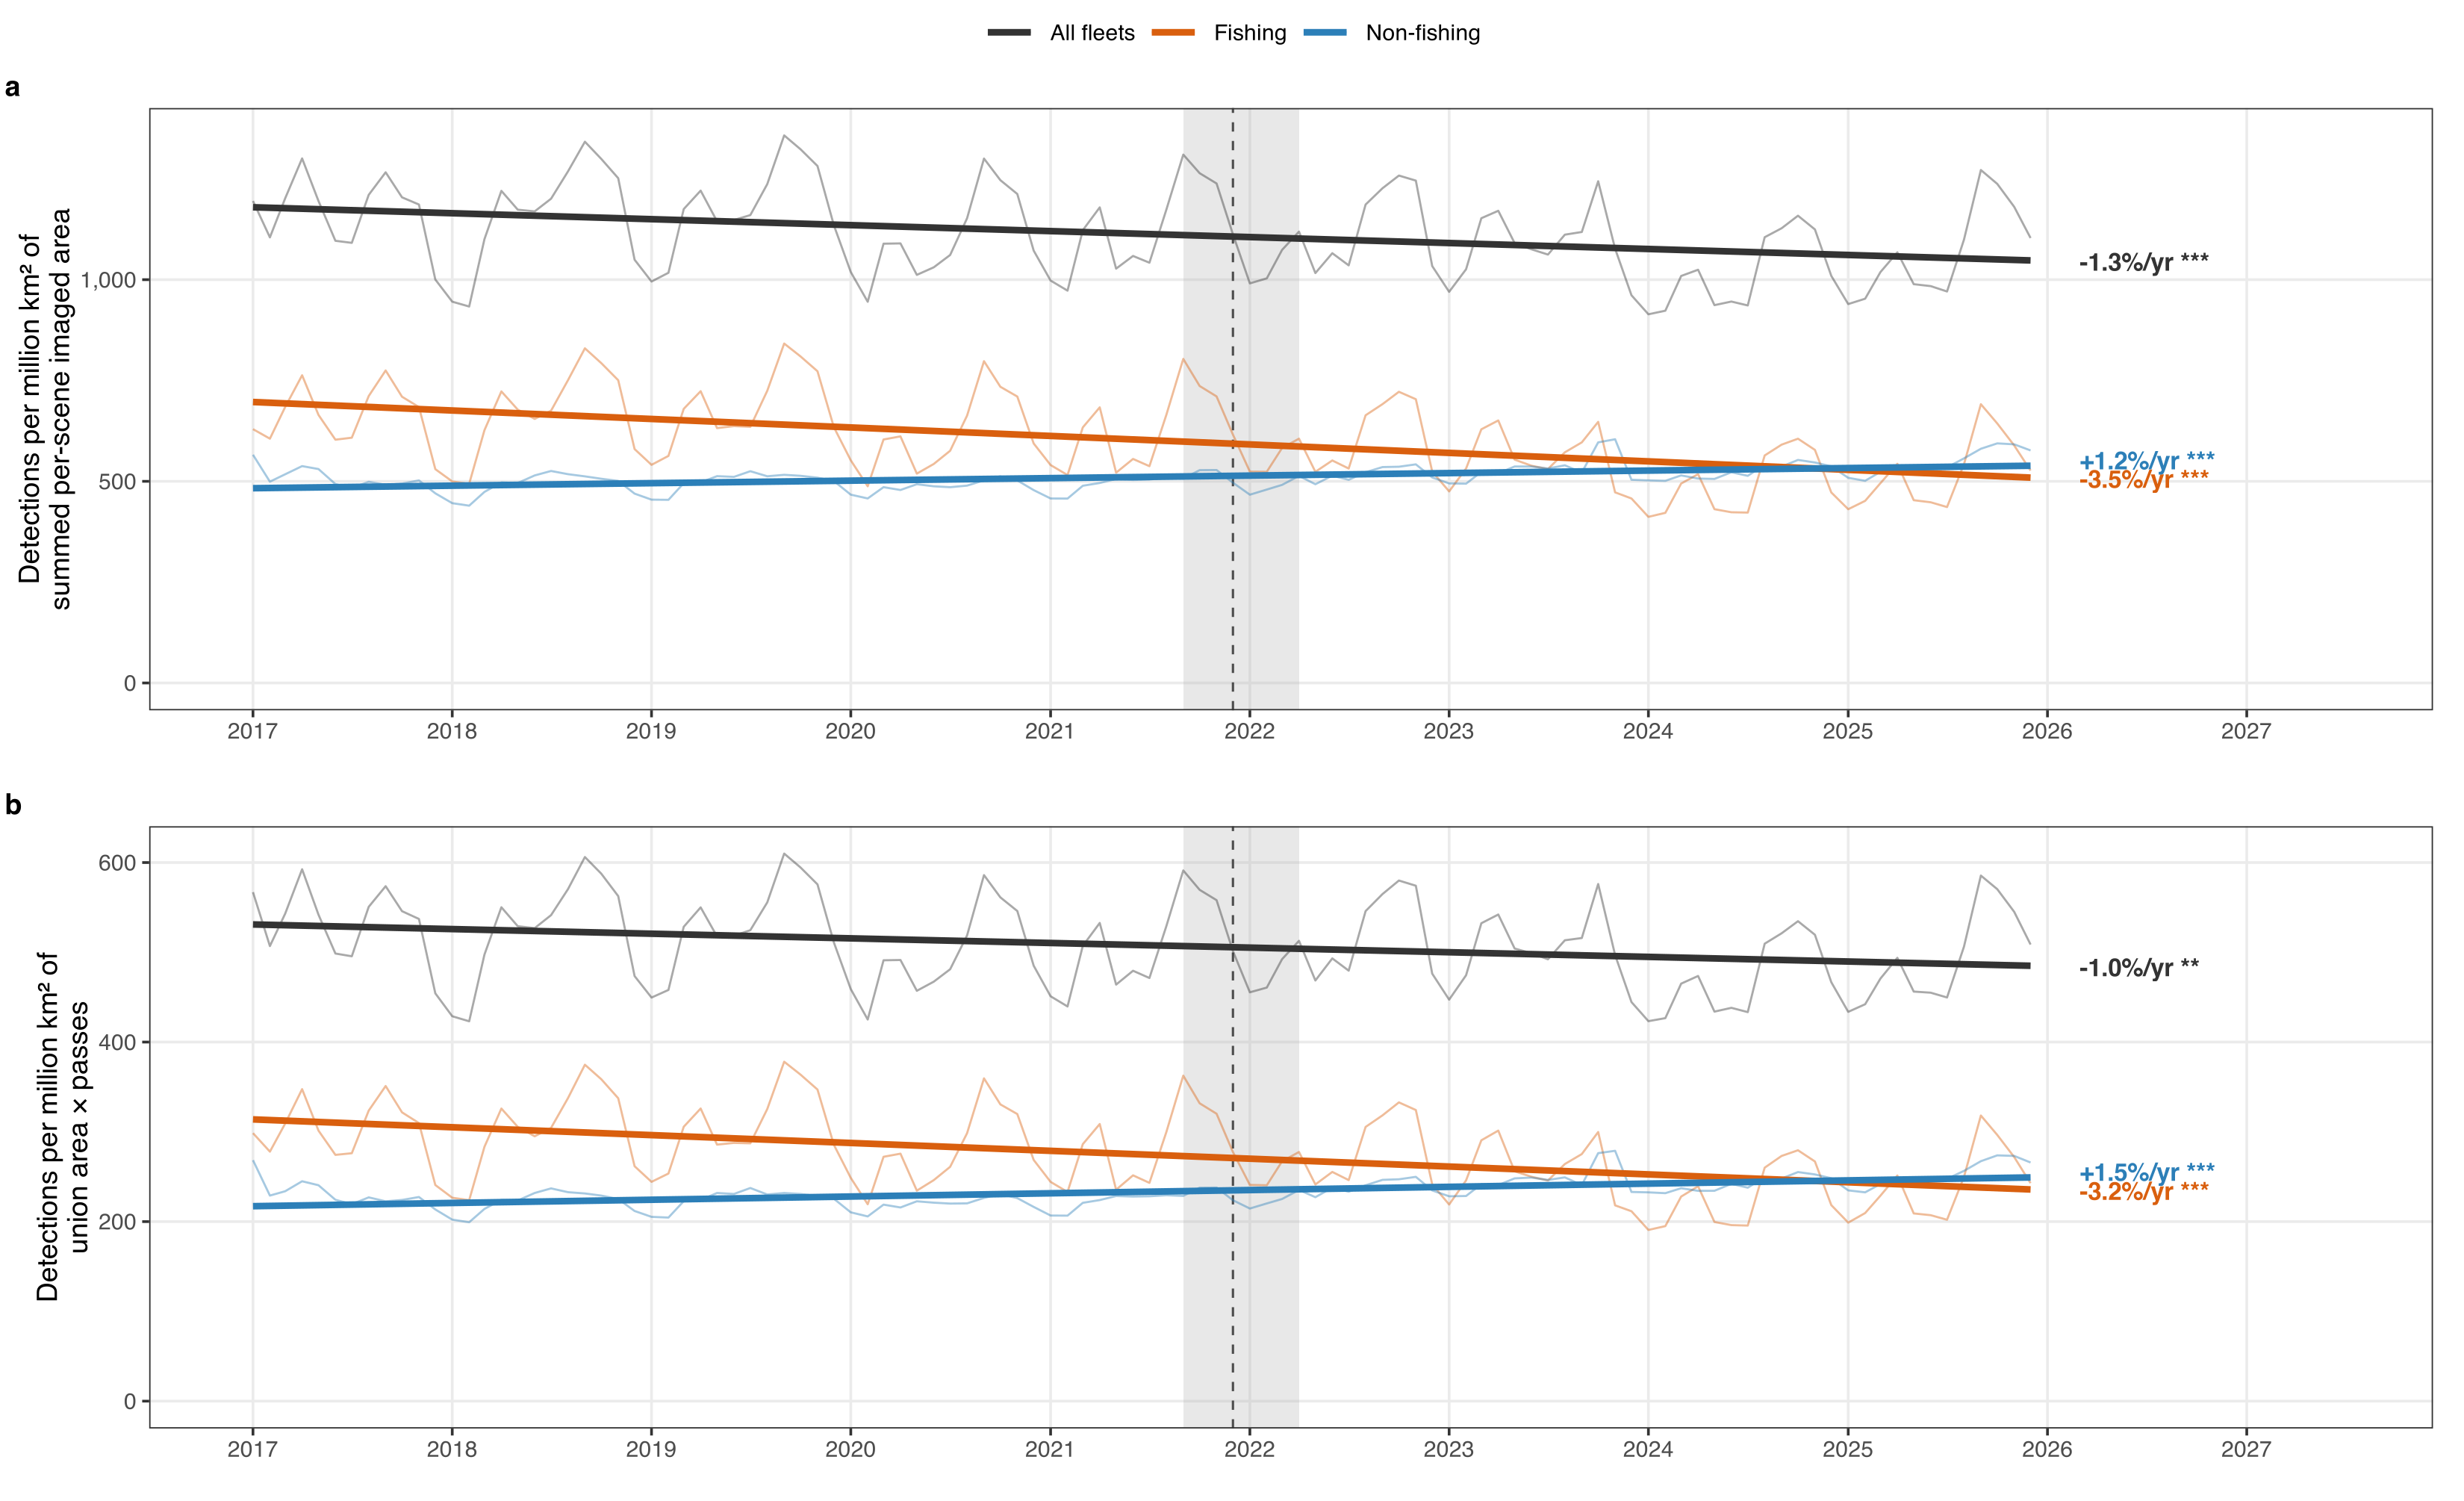
\includegraphics[width=\columnwidth]{figures/figS-density-denominators-and-bins-1.png}
    \caption{S1 detection density, 2017--2025, expressed per unit of S1 sampling effort: detections per million km² of per-scene imaged area summed across scenes, in detections per 10\textsuperscript{6} km² $\times$ pass. This is the same measure of S1 sampling effort by which our emissions models normalize their detection features, with scene footprints deduplicated before summing. Series are the fishing and non-fishing fleets and their sum. Thin lines are monthly values; thick lines are ordinary least squares fits of log density on time over the full period, labeled at the right edge with the fitted trend in percent change per year and its significance from the slope's two-sided $t$ test (*** $p<0.001$, ** $p<0.01$, * $p<0.05$, ns otherwise).}
    \label{fig:figS-density-denominators-and-bins}
\end{figure}

\begin{figure}[H]
    \centering
    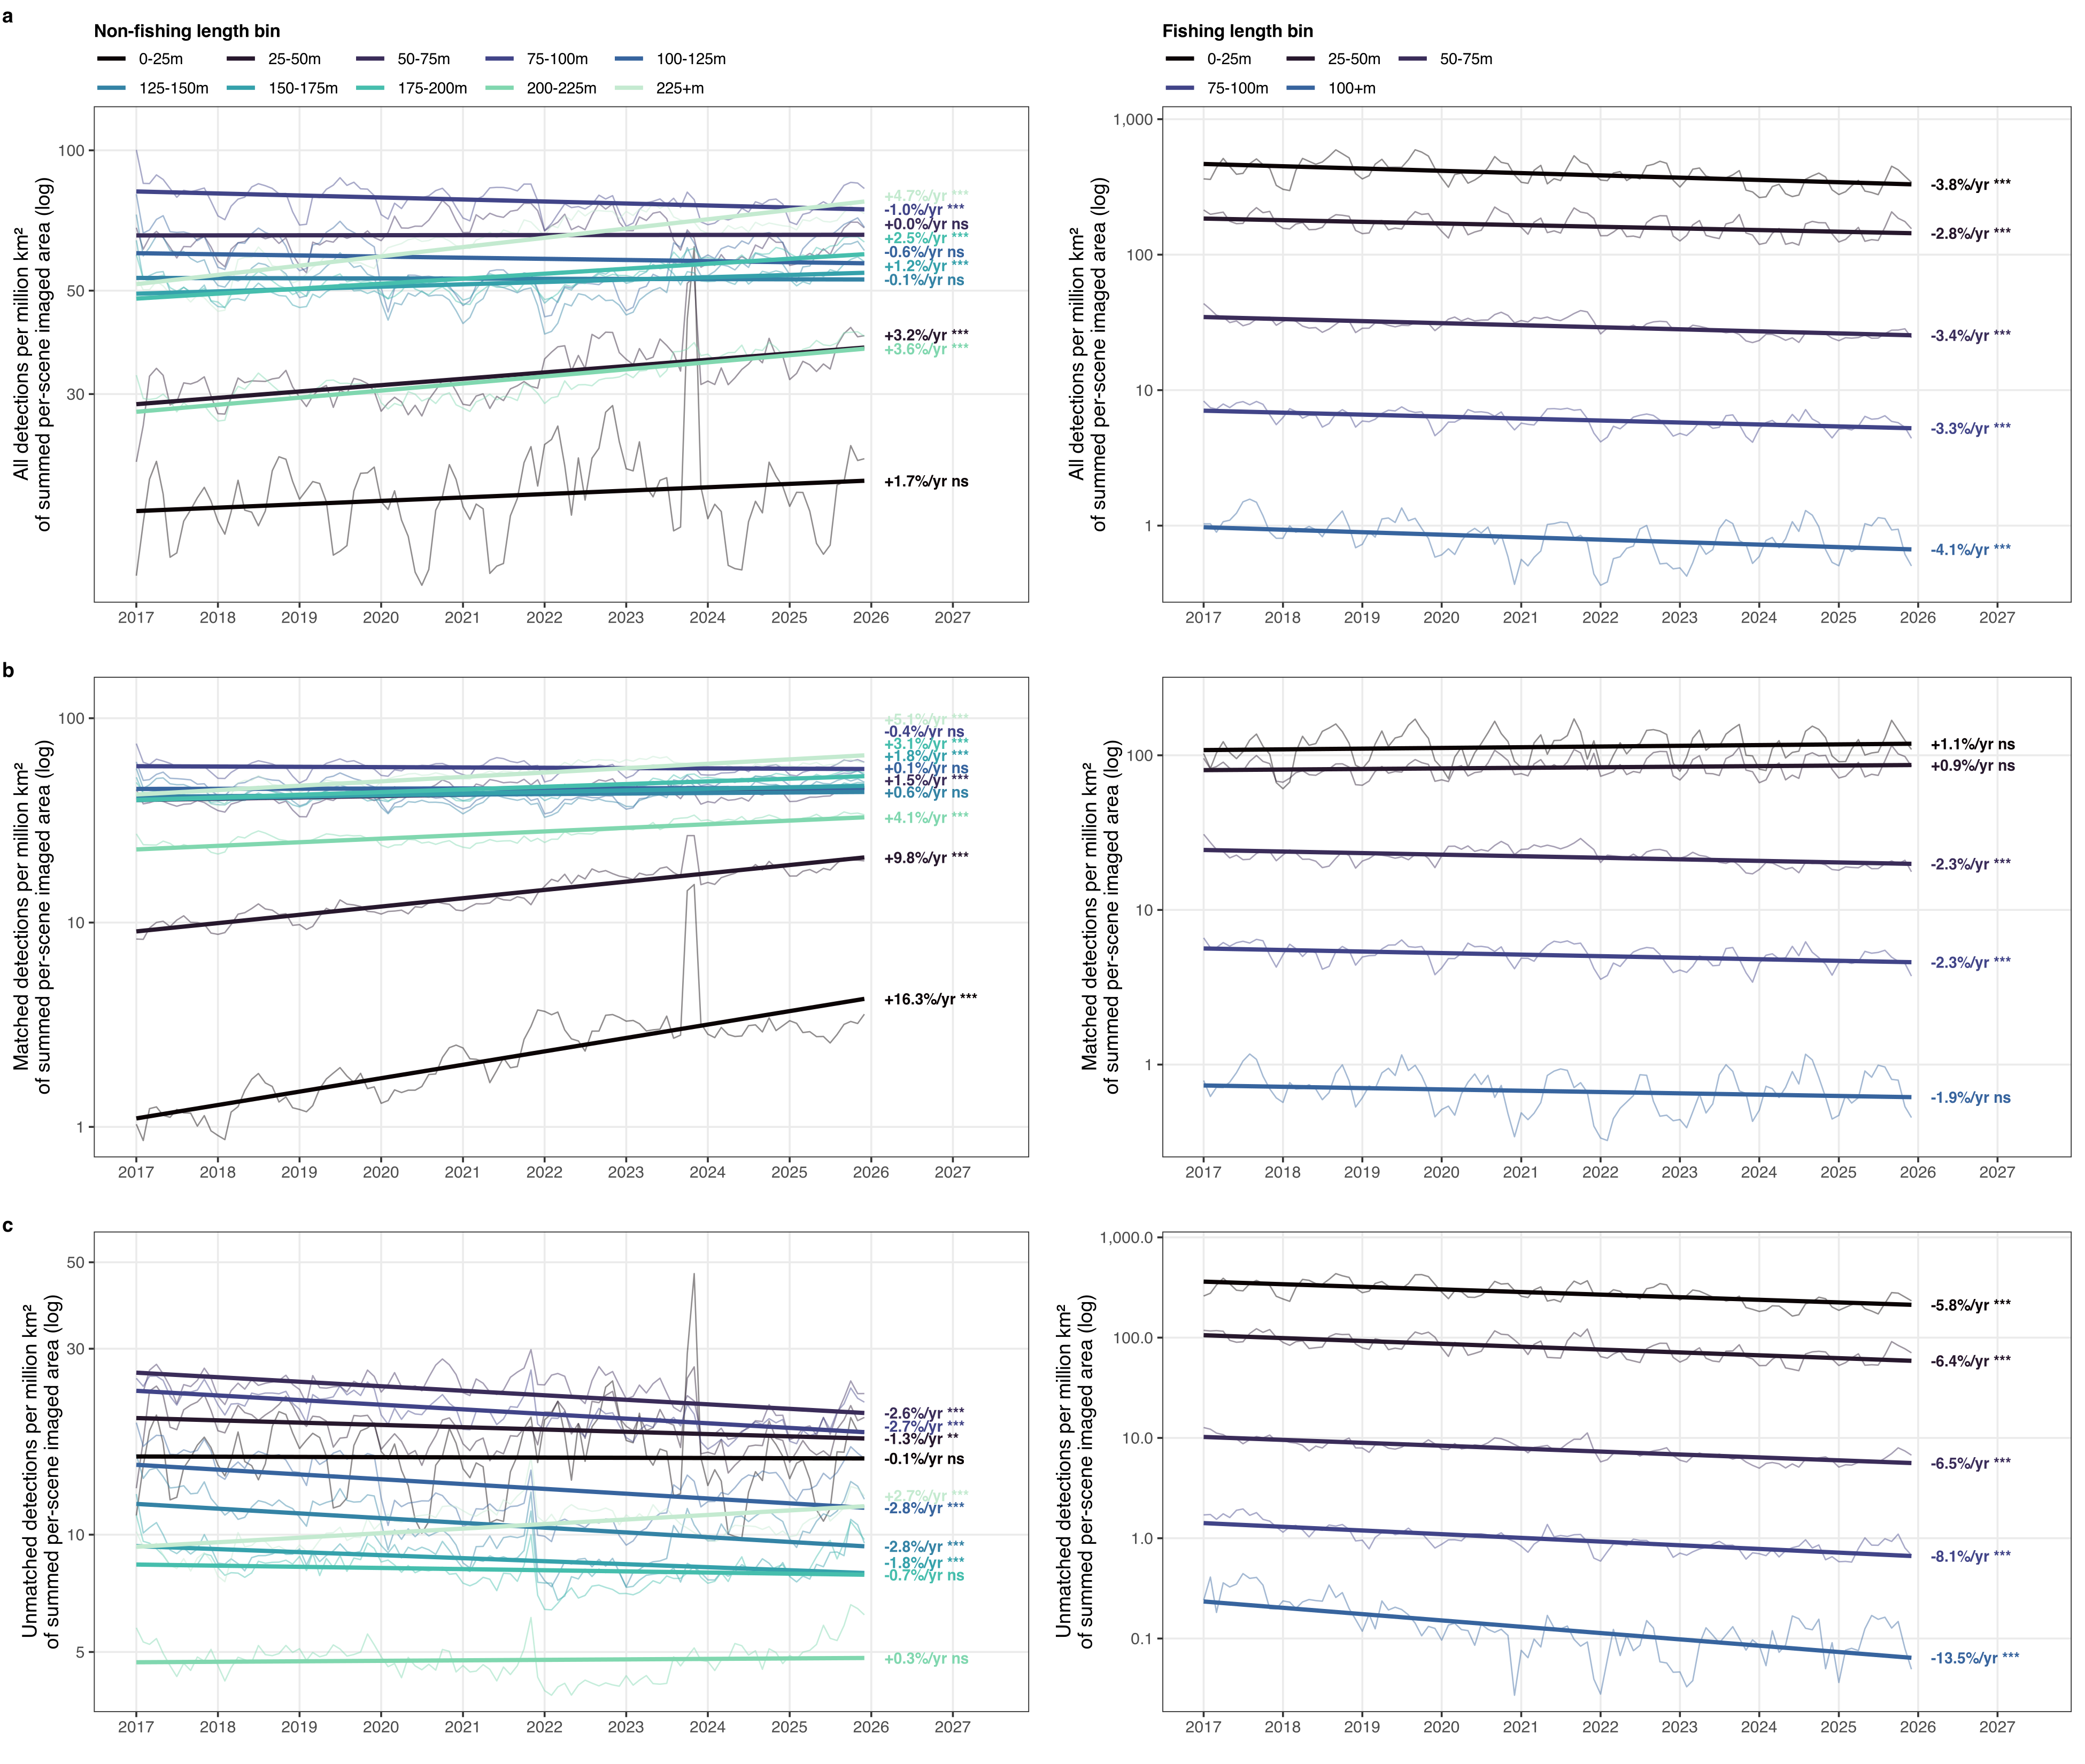
\includegraphics[width=\columnwidth]{figures/figS-density-by-match-status-1.png}
    \caption{S1 detection density by length bin, split into total, AIS-matched and unmatched detections, for fishing and non-fishing fleets. Density is expressed per unit of S1 sampling effort on the same measure used in Fig. \ref{fig:figS-density-denominators-and-bins} and by our emissions models --- per-scene imaged area summed across scenes --- so that the three series share a denominator and are additive. Axes are log scaled. Thin lines are monthly values; thick lines are ordinary least squares fits of log density on time over the full period, labeled with the fitted trend in percent change per year and its significance from the slope's two-sided $t$ test (*** $p<0.001$, ** $p<0.01$, * $p<0.05$, ns otherwise).}
    \label{fig:figS-density-by-match-status}
\end{figure}

The magnitude gap rests on firm ground: each of these mechanisms adds emissions the top-down inventories cannot account for, and our own detection limits can only mean we understate the total further. However, for the trend, whether the increase in activity explains it, depends on whether the increase reflects real activity rather than the limits of what our fused approach can observe.

Reallocation between our components requires that a vessel beginning to broadcast was already represented in the S1-unmatched estimate, and that holds only where S1 detects it. Vessels too small or too close to shore to be reliably detected, or operating outside the imaged footprint—which accounts for a fifth of our AIS emissions—contribute nothing to that component and might enter the fused total for the first time when they begin broadcasting. Because AIS carriage and reception expanded over the study period, the unobserved fraction was larger at the start of the series than at the end, so part of the measured growth in the fused total is that gap closing rather than activity rising. Figure \ref{fig:figS-density-by-match-status} (panels b and c) shows that this might be the case. Among non-fishing vessels under 25 m, matched detections (i.e., AIS-broadcasting) per unit of observing effort rise at 16\% per year while unmatched detections stay flat, so the growth there is added to the fused total rather than transferred within it. That addition could, in principle, reflect new vessels entering service. However, a 150\% increase in passenger vessels under 25 m over eight years in our AIS record (Fig. \ref{fig:figS-passenger-size-panels}) is difficult to reconcile with the idea that new construction of small craft could plausibly account for it. The more likely interpretation is that most of these vessels were already at sea but unobserved by S1, and became visible as AIS carriage and reception expanded, representing activity newly entering our record rather than newly occurring. A fused trend closely tracking the AIS-only trend is consistent with this. That the fused slope is slightly shallower indicates some genuine reallocation from the S1-unmatched component, but the similarity between the two implies that some of the measured growth enters directly through AIS rather than being transferred within the fused total.

Our fused trend is therefore likely inflated by the expansion of our own observation capacity, and is better read as an upper estimate of the underlying growth than as a measurement of it. This does not, however, imply that the flat trends of the other inventories are correct either. The reconciliation comes from the part of the fleet our approach captures without ambiguity. Among non-fishing vessels of 150 m and above, where AIS carriage is the highest and already settled at the start of our series (Fig. \ref{fig:figS-ais-carriage-saturation-by-size}), AIS-based emissions rose 29\% between 2017 and 2025, compared with 44\% for our full AIS total and 35\% for our fused total, respectively (Fig. \ref{fig:figS-registry-split-comparison}). S1 emissions are not disaggregated by vessel size, so we cannot provide the fused growth for this segment separately. The growth we report is therefore lower than our headline figure once observational expansion is set aside, but it is nowhere near the stability these inventories describe.

If these larger magnitudes and steeper trends were confirmed, the implication is not only that marine emissions have been systematically underreported, but that marine transport is among the fastest-growing sources in the global emissions picture. Our fused estimate grows roughly 4 times faster than global emissions across all sectors, and 7-9 times faster than all other transportation modes combined across EDGAR and CEDS (Fig. \ref{fig:figS-multisector-comparison}). Even confined to the segment of the fleet where observation capacity did not expand (i.e, non-fishing vessels of 150 m and above) the increase in AIS-based emissons remains more than 3 times that of global emissions across all sectors and more than 5 times that of all other transportation modes combined.

\begin{figure}[H]
    \centering
    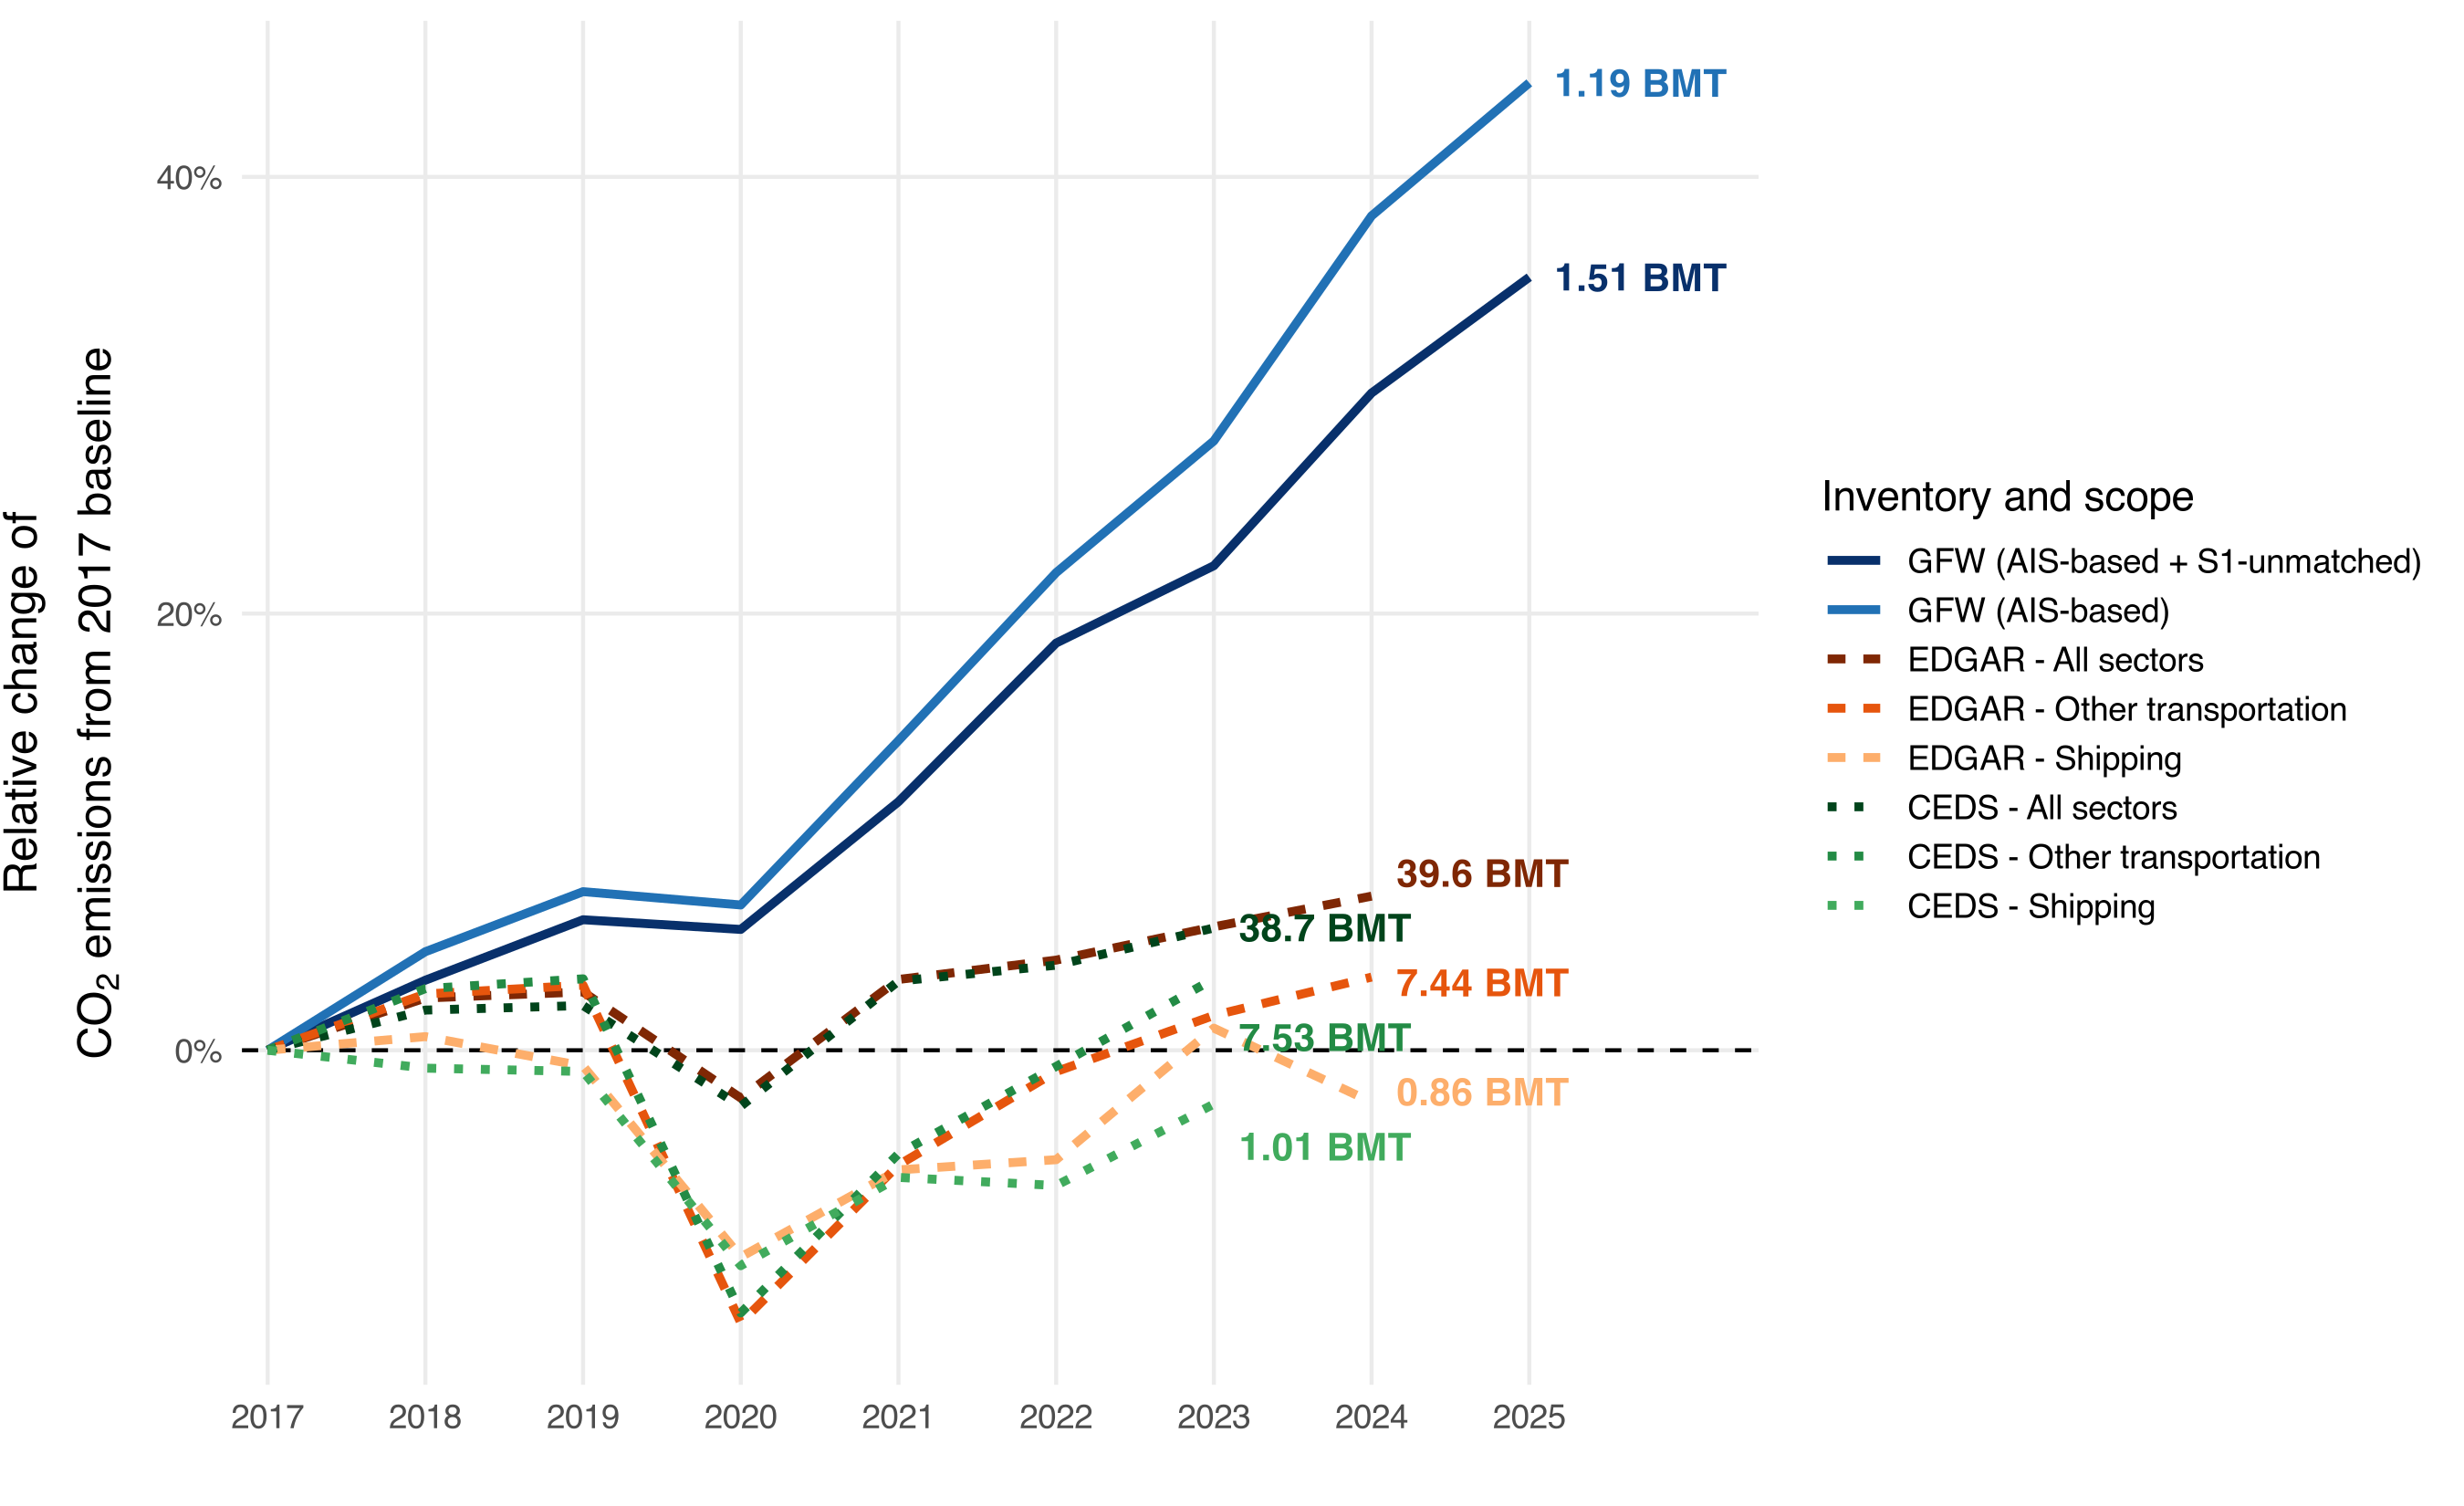
\includegraphics[width=\columnwidth]{figures/figS-multisector-comparison-1.png}
    \caption{Marine emissions growth against all sectors and against other transport modes, in EDGAR and CEDS, indexed to 2017.}
    \label{fig:figS-multisector-comparison}
\end{figure}


\end{document}
